
%\documentclass{article}
%\usepackage[utf8]{inputenc}
%%
%\usepackage{amsmath}
%\usepackage{amsfonts}
%%\usepackage{amssymb}
%%\usepackage{float}
%%\usepackage{xfrac}
%%
%\usepackage{graphicx}
%\usepackage{caption}
%%
%%
%\title{ublightcollection}
%\author{Subsection  editors:  Janet, Matt, Teppei, Gabriel, Taritree, Ben\\  Paper Editor-in-chief: Mitch}
%\date{\today}
%%
%\begin{document}
%%
%\maketitle

\section{Light Collection System}
\label{sec:light-collection}

Liquid argon is a very bright scintillator, and collecting the light produced when charged particles travel through the \lartpc is a critical aspect of fully understanding the interactions taking place in the detector.  The light collection system is designed to meet MicroBooNE's physics goals for light collection, which are twofold.
First, for accelerator-induced events, the light collection system is designed to trigger on 40~MeV kinetic energy protons produced in neutrino interactions.  Second, for non-beam events,  the system is designed for efficient observation of 5 to 10~MeV electrons from supernova neutrinos.   

The light produced by neutrino interactions in MicroBooNE is an important input for both event selection and reconstruction.  
One of the critical capabilities the light collection system provides is the ability to form a beam-event trigger when a pulse of light is observed in coincidence with the beam spill.  Because a vast majority of beam spills will not produce a neutrino interaction in the detector, such a trigger will substantially reduce the data output rate.  
For non-beam physics studies, the light system provides triggering and an event $t_0$. For accelerator-induced events, the start time of a beam spill is, in principle, sufficient.  
However, because of the long window over which the ionization electrons of an event drift (about 1.6 ms maximum drift time at 500 V/cm field), there are many accelerator-induced events in which a cosmic ray muon crosses the detector during the drift time.  Utilizing the position of hits in the photodetectors, one can better reject cosmic ray muon tracks.  
The light can also be used to trigger and select specific types of cosmic-ray calibration events (Michel electrons, straight-through muons, etc.) and non-beam events (supernova neutrinos, cosmic background events to proton decay studies, etc.).

The light collection system consists of primary and secondary sub-systems.  The primary light collection system is made up of ``optical units,'' each one consisting of a PMT located behind a wavelength-shifting plate.  In total, 32 optical units were installed, yielding 0.85\% photocathode coverage.  The secondary system consists of four light guide paddles.   These paddles are introduced for R\&D studies for future LArTPCs, and are placed near the primary optical units to allow a comparison of their performances.  A flasher system, used for calibration, consists of optical fibers bringing visible light from an LED to each PMT face.

The light collection detectors are located in the $y$-$z$ plane behind the anode planes of the LArTPC, as shown in figure~\ref{fig:lightlayout}.  The combined transparency of the three anode planes is 86\% for light at normal incidence.  This transparency value assumes 100$\%$ of VUV photons impinging on the wires (150 $\mu$m diameter and 3 mm pitch) are absorbed.  The detectors were placed so as not to be obscured by the \lartpc structural cross-bars, shown in figure~\ref{fig:lightlayout}.  Locating the light detectors behind the anode plane places them in a very weak electric field due to the +440 V bias of the collection plane.  To test for an effect from weak electric fields, the response of a PMT placed between a +700 V mesh and ground, separated by 50 cm, was studied.  The PMT zenith was 25 cm from the HV.   No effects on the signal were observed.  This was expected, as the photocathode is held at ground, effectively acting as a Faraday cage.  
%: $(1-0.150/3)^3 = 86\%$. 

Throughout the design and construction of the light collection system,  substantial R\&D was performed.   The reader should refer to~\cite{Jones:2013bca,Bugel:2011xg,Katori:2011uq,Chiu:2012,Baptista:2012,Briese:2013wua,Jones:2013mfa,Katori:2013wqa,Moss:2014ota,Conrad:2015xta,Moss:2015hha} for detailed results of these studies.    A useful overall review is available in~\cite{Jones:2015bya}. 

Figure~\ref{fig:muondecaylight} shows the light observed in two sequential events, consistent with a muon entering the detector followed by a Michel electron from the decay.   One can see that the light is relatively well localized.   This allows the light to be correlated with specific tracks in the detector.  This ``flash-track matching'' is used to identify and reconstruct the tracks that are in time with the beam spill--an important goal of the light collection system.


\begin{figure}[t]
	\centering
%       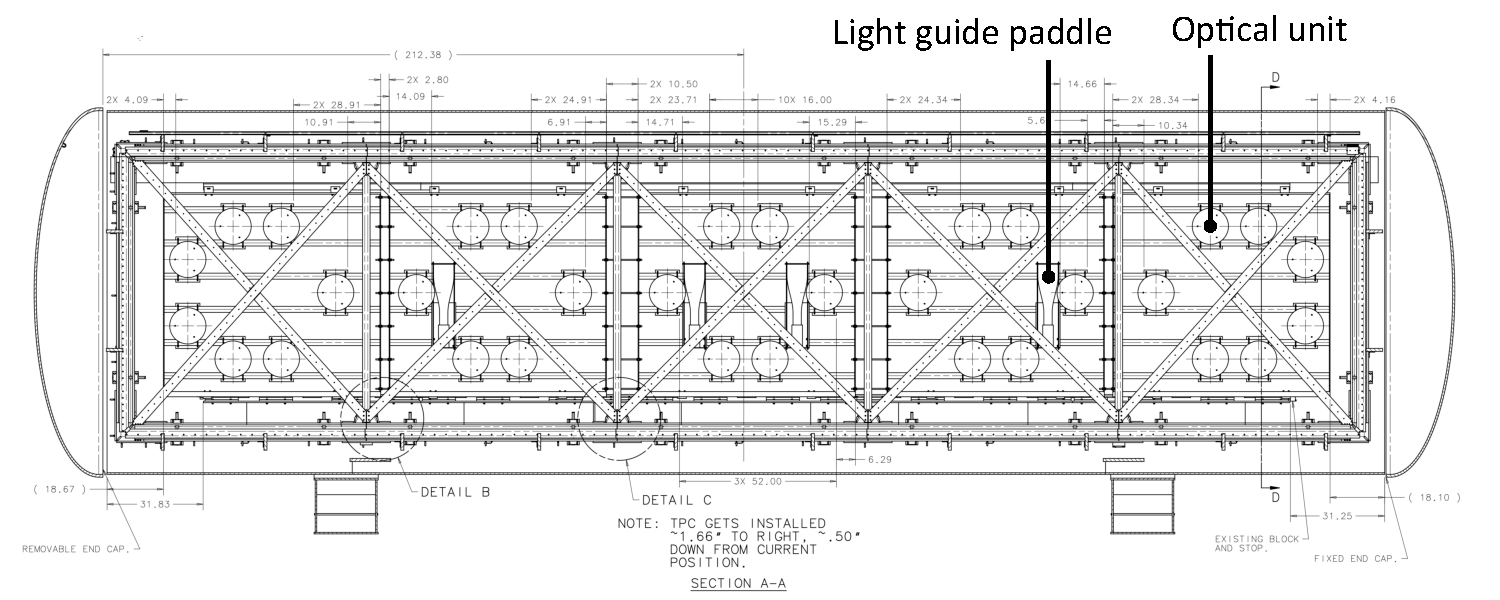
\includegraphics[width=0.95\textwidth]{./light_figures/PMTPlacement.pdf} 
              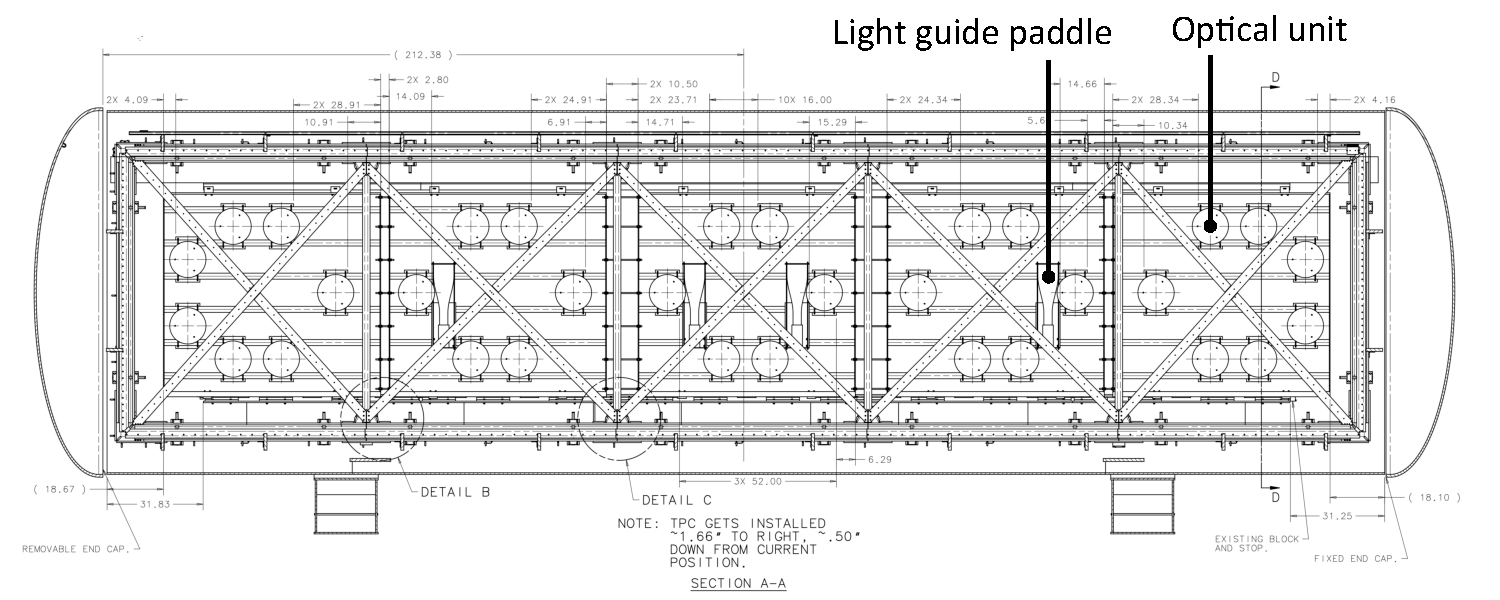
\includegraphics[width=0.95\textwidth]{./light_figures/PMTPlacement.pdf} 
        \caption{The MicroBooNE light collection system consists of a primary system of 32 optical units and a secondary optical system of four lightguide paddles~\cite{Katori:2013wqa}. These are mounted behind the anode wire planes such that the view is not obscured by structural cross bars of the LArTPC. }\label{fig:lightlayout}
\end{figure}

\begin{figure}[t]
	\centering
    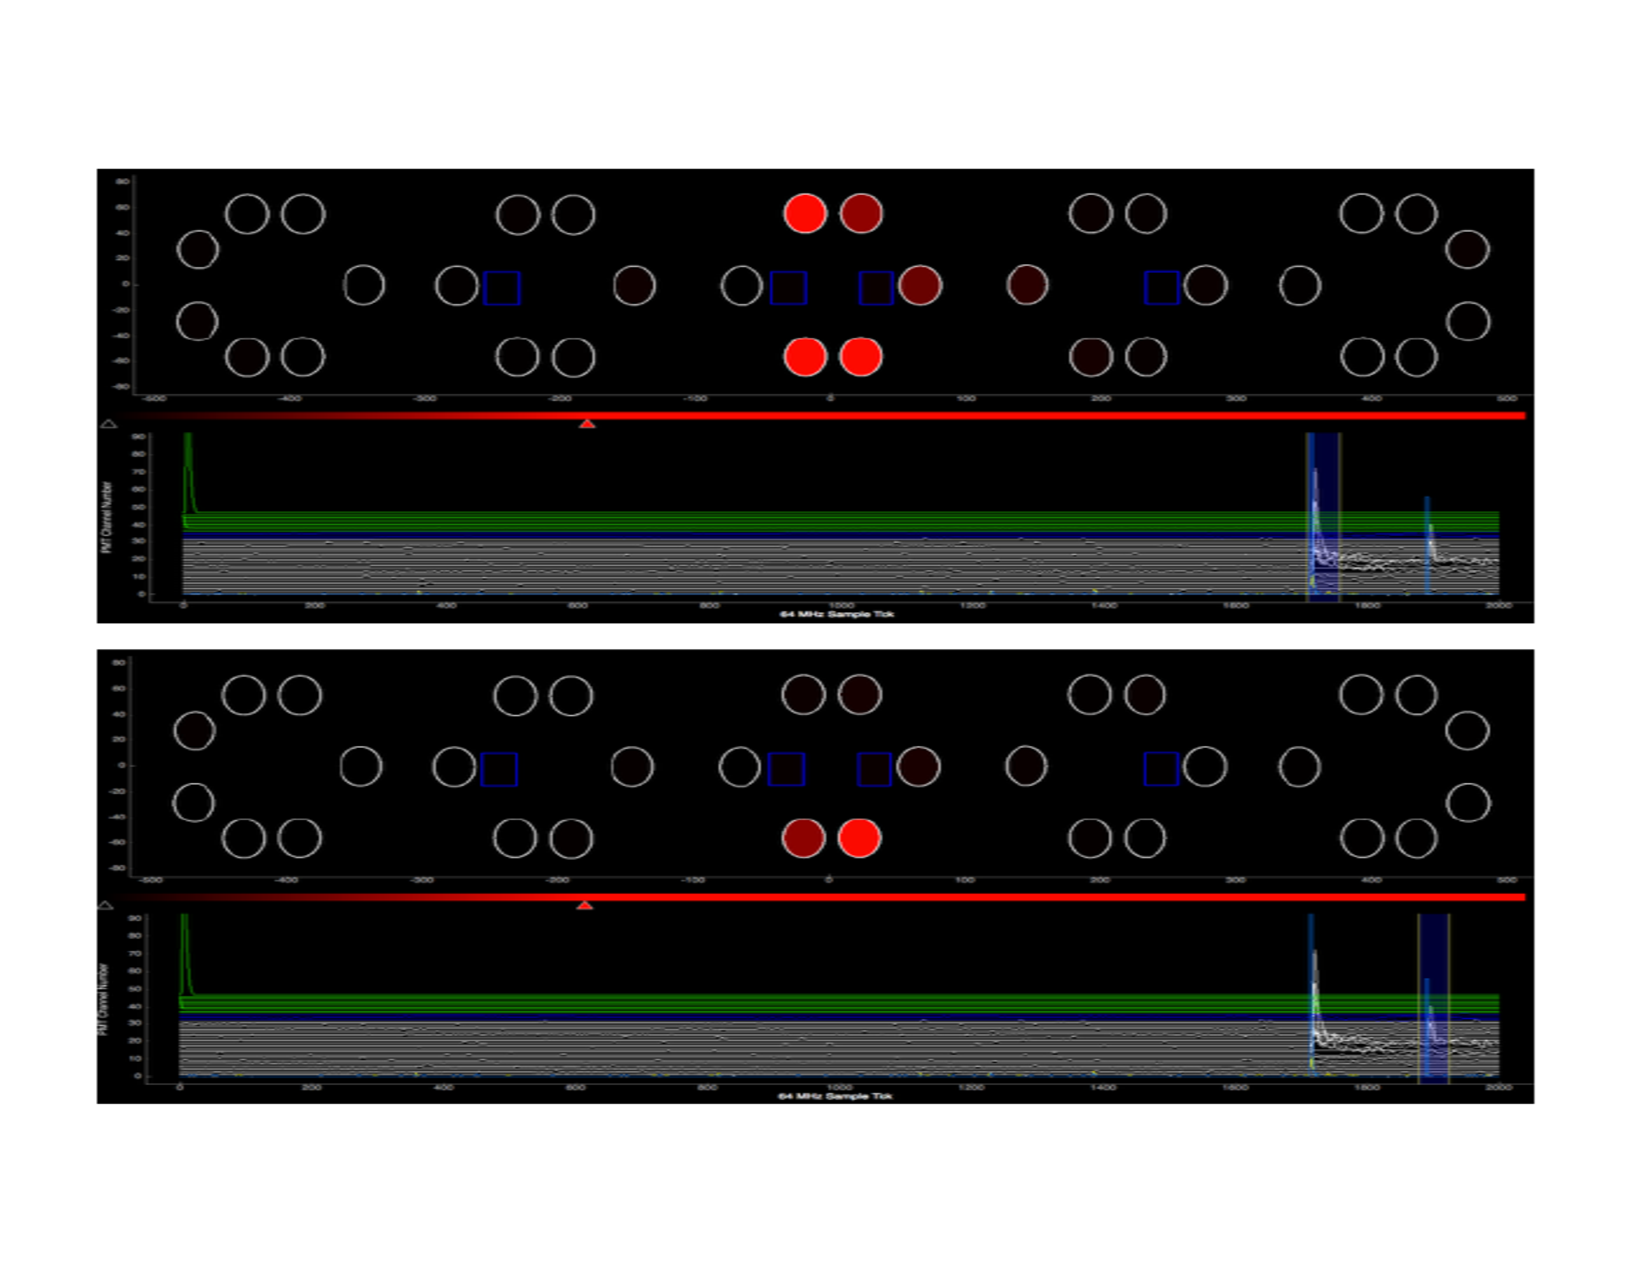
\includegraphics[width=0.95\textwidth]{./light_figures/muondecay.pdf} 
    \caption{Two sequential event displays for the light collection system.  The sequence is consistent with a muon that stops (top) and decays (bottom).  The circles correspond to the optical units. Red circles indicate those units with hits.    The waveforms versus time are shown below.}\label{fig:muondecaylight}
\end{figure}


\subsection{Light Production in Argon \label{sint}}




\begin{table}[t]
   \centering
    \caption{Important properties of scintillation light in liquid argon that affect detection in MicroBooNE.} 
    \begin{tabular}{llr} % Column formatting, @{} suppresses leading/trailing space
    \hline
    Property & Value & Reference\\
    \hline
    Wavelength & 128 nm & \cite{SUZUKI1979197}\\
    Singlet, Triplet state time constants & 6 ns, 1.6 $\mu$s &\cite{PhysRevB.27.5279} \\
    Photons/MeV for $E=500$ V/cm & 24000 & \cite{Amerio:2004-T600}\\
     Triplet lifetime quench due to N$_2$ at 1 ppm  & 20$\%$ & \cite{Acciarri:2008kv} \\
     Attenuation length due to N$_2$ at 1 ppm & 66 m &\cite{Jones:2013bca} \\
     Rayleigh Scattering Length & $\sim$90 cm &\cite{1997NIMPA.384..380I} \\
     Transparency of the wireplanes at normal incidence & 86$\%$ & -\\
    \hline
   \end{tabular}
   \label{tab:lightparam}
\end{table} 

Light produced in liquid argon arises from two processes: scintillation and Cherenkov radiation.  
Scintillation light is produced by the formation and eventual radiative decay of excited argon dimers (or eximers) and is emitted in an isotropic distribution.  Liquid argon is an excellent scintillator: it produces a large amount of light per unit energy deposited (about 24,000 photons per MeV at 500 V/cm drift field) and is transparent to its own scintillation. %Scintillation light dominates the Cherenkov radiation by a factor of five and thus represents the bulk of the light detected.
The scintillation light has a prompt and slow component with decay times of about 6 ns and 1.6 $\mu$s, respectively. The two lifetimes correspond to the two lowest-lying eximer states with the prompt component coming from the decay of a singlet state and the slow from the decay of a triplet state.  The prompt to slow ratio is about 1:3 for minimum ionizing particles and varies with ionization density and particle type. Both components consist of photons with a wavelength of 128 nm.

There is a significant uncertainty on the expected triplet lifetime \cite{PhysRevB.27.5279} and this may be further modified by quenching (non-radiative dissociation of excimers by impurities)  \cite{Acciarri:2008kv}.  Other factors that can affect the arrival of the light include Rayleigh scattering, absorption by impurities, and obstructions.  For detailed discussion of the physics of scintillation light production and propagation in MicroBooNE, see~\cite{Jones:2015bya}. Table~\ref{tab:lightparam} summarizes information about the scintillation light.  

\begin{figure}[t]
	\centering
%       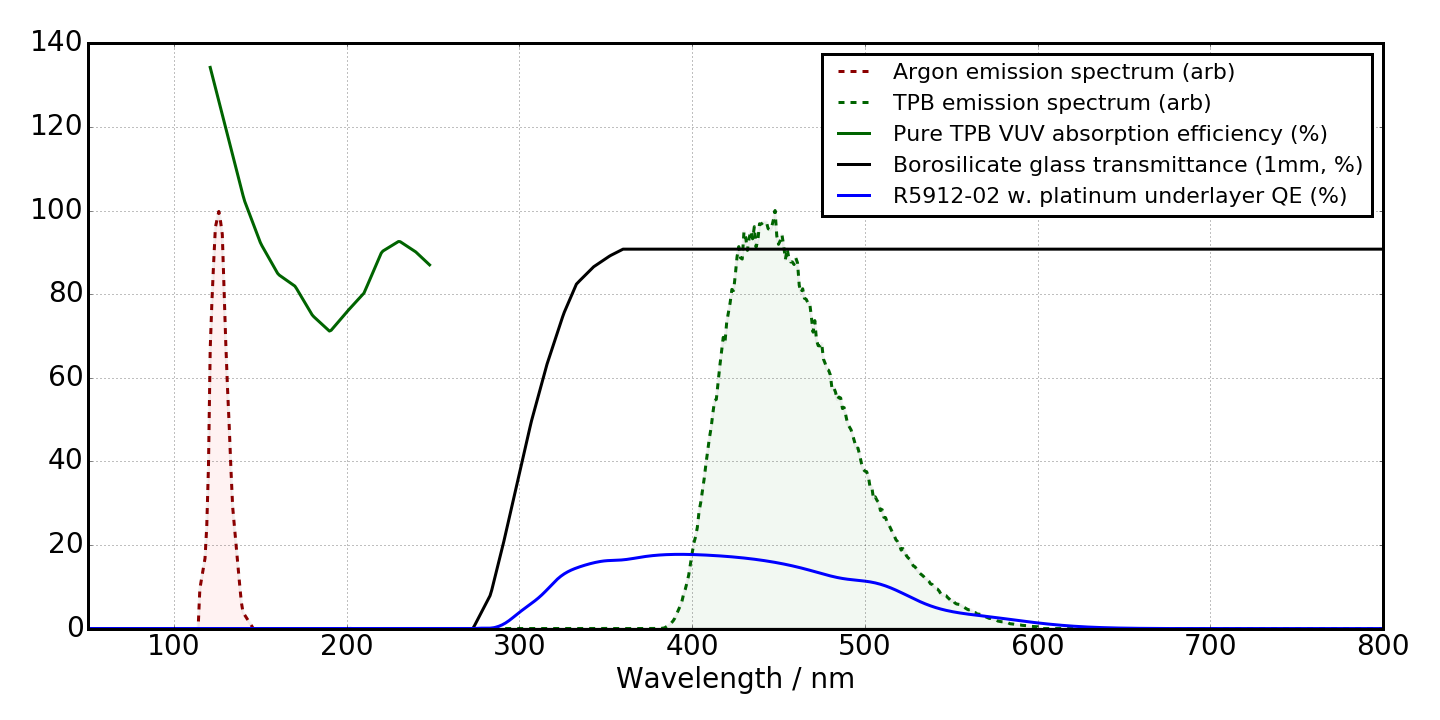
\includegraphics[width=\textwidth]{./light_figures/pmttpbeff.png}  
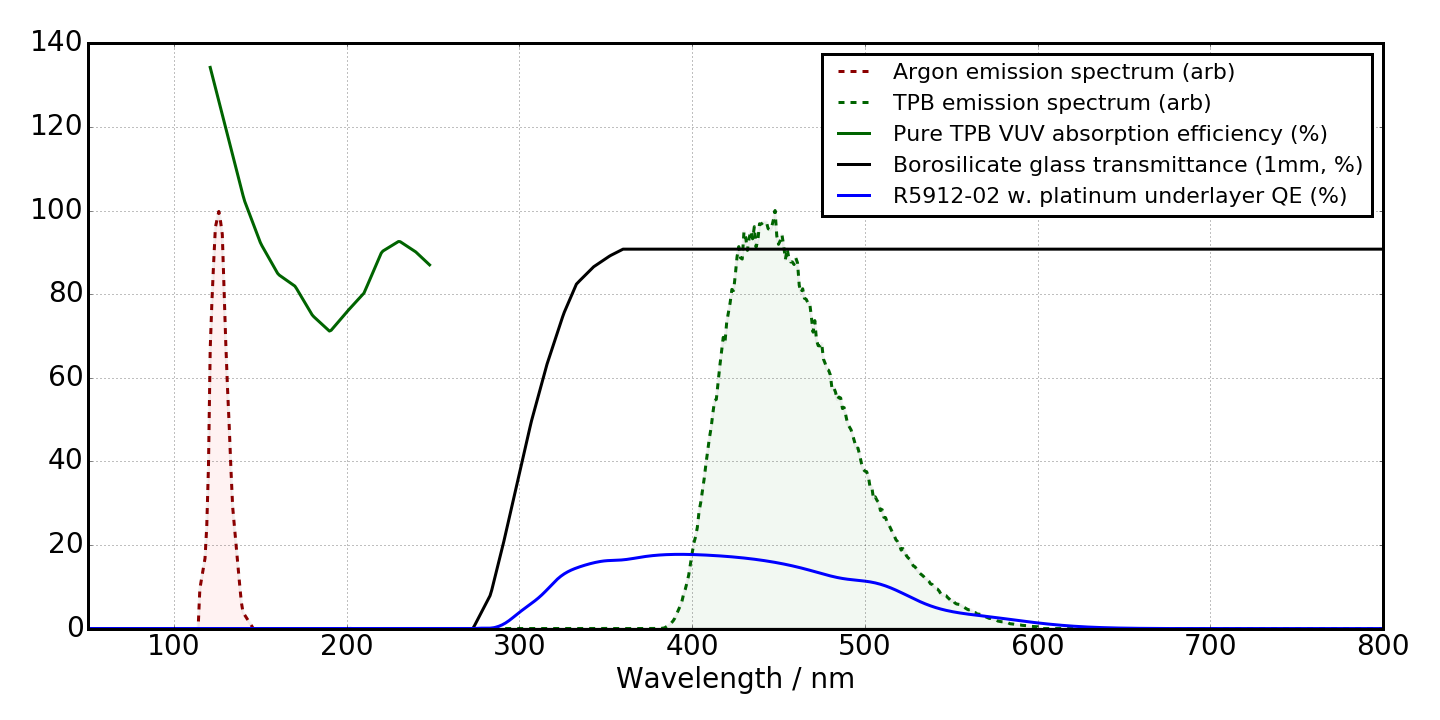
\includegraphics[width=\textwidth]{./light_figures/pmttpbeff.png} 
        \caption{Scintillation light emission spectrum (red) and TPB re-emission spectrum (green), in arbitary units.  Superimposed are important efficiencies (see $y$ axis):  Dark green line -- absorption of VUV light by TPB;  Black line -- transmission of borosilicate glass;  Blue line -- efficiency of a R5912-02mod cryogenic PMT \cite{Jones:2015bya} }\label{fig:lightchallenge}
\end{figure}


Because scintillation photons have a wavelength of 128 nm they are are very difficult to detect using conventional photodetectors.  Figure~\ref{fig:lightchallenge} summarizes the challenges involved in detection of the 128 nm scintillation light.  
In order to detect the scintillation light, with spectrum shown in red, the VUV photons must be shifted into the visible region.   MicroBooNE employs tetraphenyl-butadiene (TPB).
This organic fluor absorbs in the UV (green line) and emits in the visible with a peak at $425\pm20$~nm (green hatched region), the peak wavelength having a slight dependence on the micro-environment of the fluors.  This is a favorable wavelength for detection by the PMTs employed by MicroBooNE.  The efficiency for transmission through borosilicate PMT glass (black) and the quantum efficiency of the cryogenic tubes used in MicroBooNE (blue) are overlaid on the TPB spectrum.

%\subsection{Light Collection System Overview}


%\begin{table}[~htb]
%   \centering
%    \caption{Light Collection parameters for MicroBooNE.} 
%    \begin{tabular}{lcr} % Column formatting, @{} suppresses %leading/trailing space
%    \hline
%    Parameter & Value & Note\\
%    \hline
%     PMTs & 32 8'' Hammamatsu R5912-02mod & Photocathode coverage to trigger on 40 MeV protons.\\
%     Scintillator Paddles & 4 & R$\&$D\\
%     High/Low Gain & Energy & \\
%     Timing & & \\
%    \hline
%   \end{tabular}
%   \label{tab:lcdetparam}
%\end{table} 

\subsection{The Primary Light Collection System}

\begin{figure}[t]
	\centering
           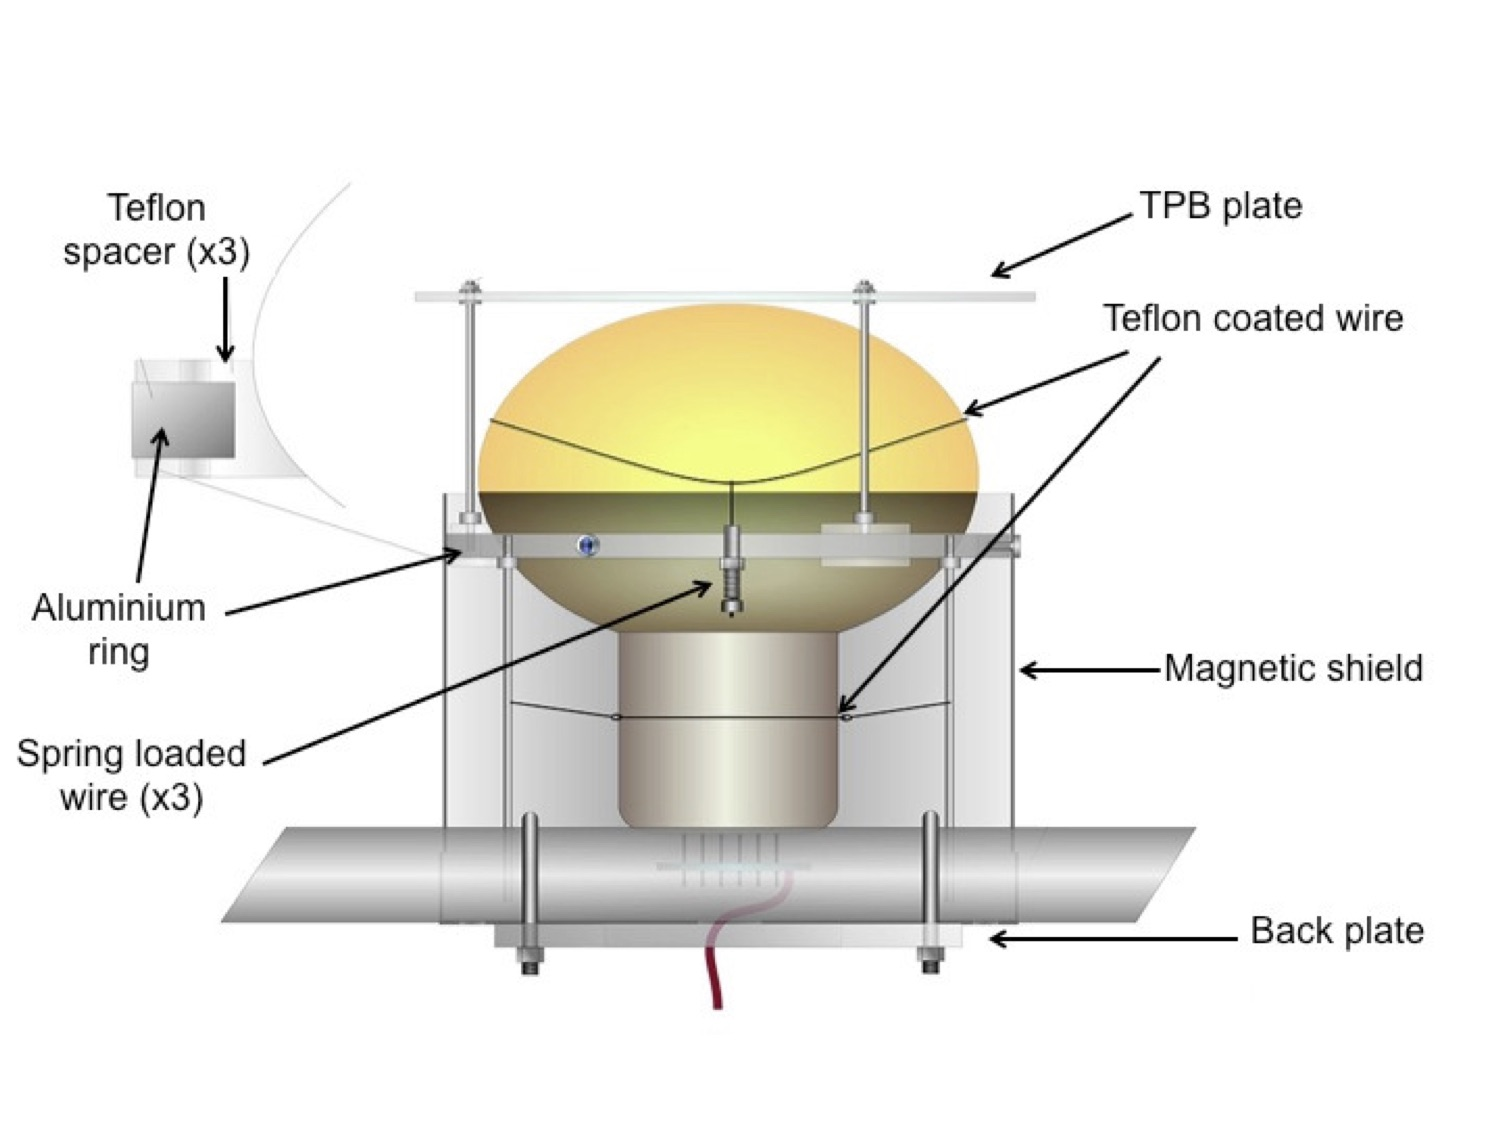
\includegraphics[width=0.45\textwidth]{./light_figures/PMTmount2.jpg} 
           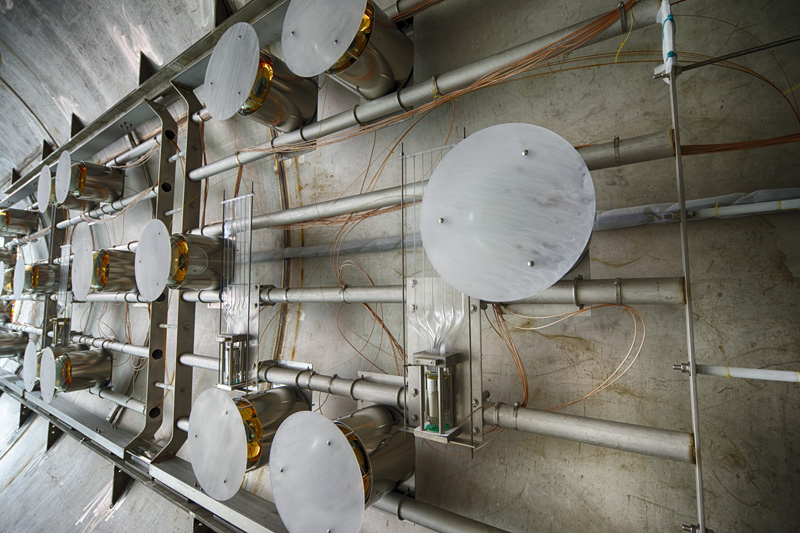
\includegraphics[width=0.45\textwidth]{./light_figures/13-0430-05D.jpg} 
        \caption{Left: diagram of the optical unit; Right: units mounted in MicroBooNE, immediately prior to \lartpc installation.}\label{fig:unitmounted}
  %}%
  %\fbox
\end{figure}


Each of the 32 optical units of the primary light collection system consist of a cryogenic Hamamatsu 5912-02MOD PMT seated behind an acrylic plate coated with a TPB-rich layer and surrounded by a mu-metal shield. 
Figure~\ref{fig:unitmounted} shows a diagram of one unit (left) and a photograph of installed units (right).  Past experiments have directly coated PMTs with wavelength shifter \cite{Amerio:2004-T600}.  However, 
the MicroBooNE design separates the PMT from the wavelength-shifting plate for simplicity of quality control and installation.  This proved important, as R\&D indicated that TPB is particularly vulnerable to environmental degradation (see section~\ref{environ}).  In this section, description is provided for each component of the optical unit, as well as for the overall assembly.


\subsubsection{Photomultiplier Tubes and Bases}
\label{sec:pmt-bases}

Reference \cite{Briese:2013wua} provides detailed information on the selection 
and testing of the 8" Hamamatsu R5912-02mod cryogenic PMTs employed in MicroBooNE.   
In this section a brief summary of the findings from this testing is presented.

The R5912-02mod employs a bi-alkali photocathode.  Because the PMT is designed for cryogenic use, the R5912-02mod also features a thin platinum layer between the photocathode and the borosilicate glass envelope to preserve the conductance at low temperatures.   While this allows the PMT to function below 150 K, absorption in the platinum reduces the efficiency of the PMT by 20\%.
Figure \ref{fig:TPBSpectraPlate} provides quantum efficiency curves for the 8 inch PMTs. The manufacturer's specifications do not include the effects of the platinum photocathode coating, but a wavelength dependent quantum efficiency was provided by Hamamatsu for 4 of the 32 installed PMTs.  The mean and standard deviation of these curves are shown in figure \ref{fig:TPBSpectraPlate}. 

The  R5912-02mod is a 14-stage PMT.
The high gain at room temperature ($10^9$ at $\sim$1700 V), compensates for known reduced gain at 87 K in the liquid argon.  
The high gain also has the additional advantage of allowing operation at lower than nominal voltage which reduces heat-loss in the cables and the potential for high voltage breakdown at the feedthroughs.


\begin{figure}[t]
\centering 
%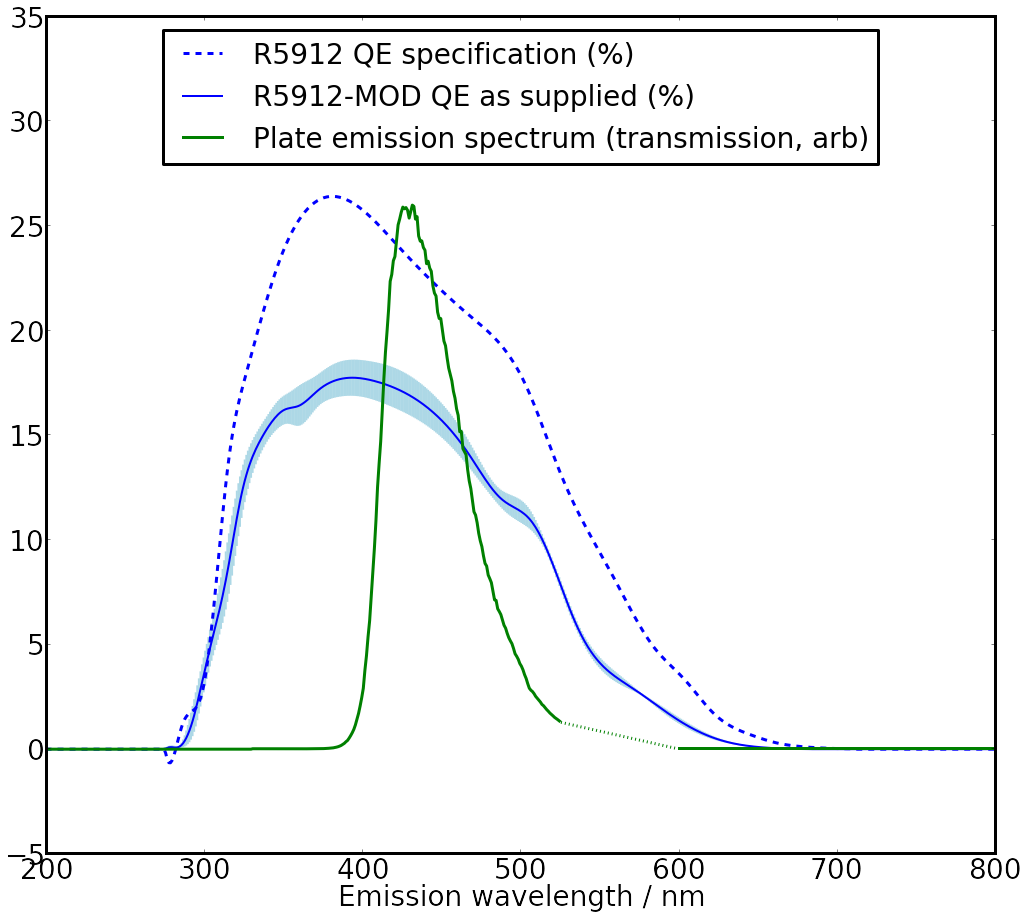
\includegraphics[width=0.65\textwidth]{./light_figures/PlateSpectra.png}
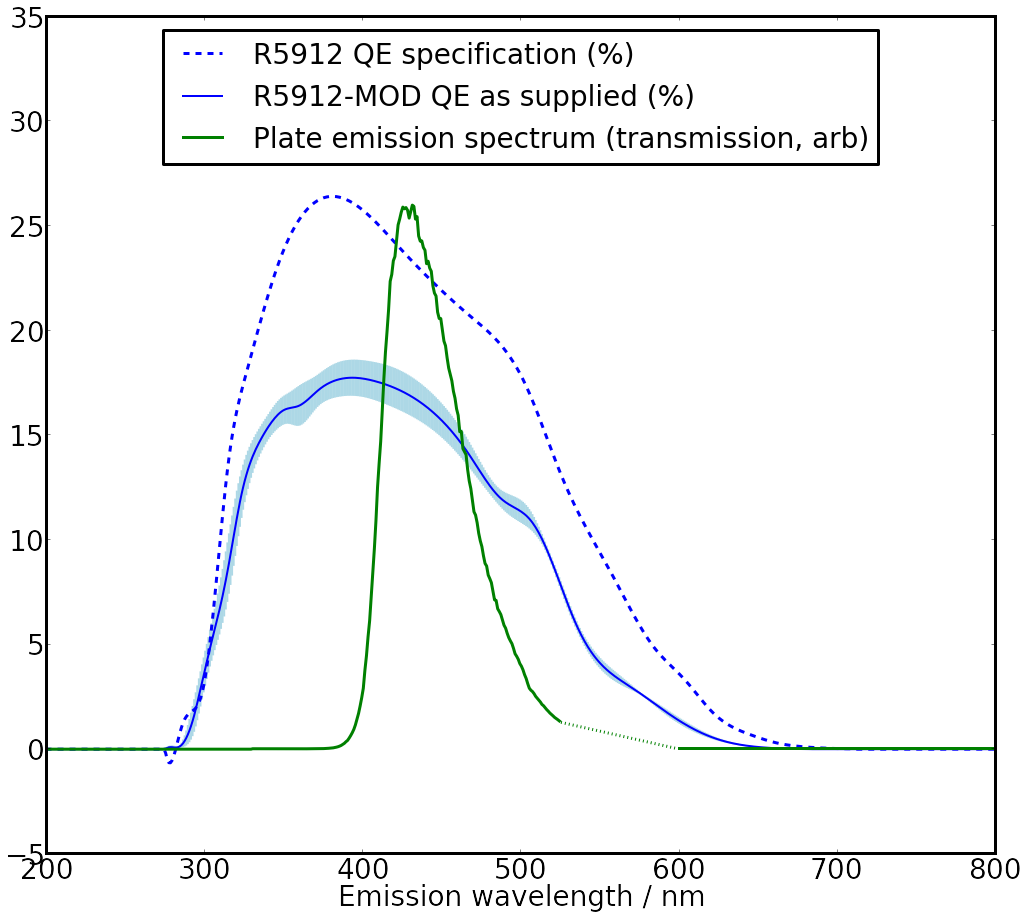
\includegraphics[width=0.65\textwidth]{./light_figures/PlateSpectra.png}
\caption{The specification for the non-platinum undercoated PMT from \cite{Hamamatsu-Datasheet8inch}.  The blue band shows the mean and standard deviation of the four quantum efficiency curves provided by Hamamatsu for installed MicroBooNE PMTs. Also shown is the measured emission spectra of MicroBooNE wavelength-shifting coatings, discussed in section \ref{sec:wavelengthshift}.  \cite{Jones:2015bya}
 \label{fig:TPBSpectraPlate}  }
\end{figure}


The PMT base is designed such that the photocathode is 
grounded and the last dynode in the chain is held at large, positive voltage. 
Thus the PMT bulb, which is closest to the \lartpc anode plane, 
is at ground and does not disturb the electric field on the wires.  
The result is that the high voltage (HV) can be provided and the signal can be extracted from the PMT using a single cable, 
reducing the cable volume in the vapor region and removing a possible source of out-gassing water impurity.

The flat PC-board base was made of Rogers RO4000-series woven glass-reinforced laminate, 
which is the same material with the \lartpc cryogenic front end boards.  Use of Rogers 4000 series as the base material avoids the potential risk of contamination of the liquid argon. The Rogers material has a similar temperature expansion coefficient as the surface mounted components which enhances the reliability of the electronics assembly when operated at cryogenic temperatures.  The base is attached $\sim 1$ cm from the bottom of the PMT and is the closest possible distance of safe approach to the PMT vacuum seal tip.   
A schematic and photos of the PMT base are provided in reference~\cite{Briese:2013wua}. 
The passive components include only metal film resistors and C0G/NP0 capacitors, 
which have the minimum temperature coefficients, and the performance at cryogenic temperatures were tested.  
Because the supplied HV and return signal share a single cable, the signal must be split from the HV through an AC-coupling capacitor, as is discussed in section~\ref{LCUnitimplement}.

All installed PMTs were tested in a PMT test stand, both
at room temperature and in liquid nitrogen which is at 77 K.  
%Figure~\ref{fig:PMTteststand} shows a drawing of the PMT test stand. 
The details are described in reference~\cite{Briese:2013wua}.  
In brief, the test stand consisted of a light-tight 346~L, 
liquid nitrogen filled dewar into which up to four PMTs could be installed. 
The PMTs were immersed and maintained in the dark environment 
for up to three days before most measurements of the dark rate and gain were performed.  
A fiber brought in light from a pulsed blue LED, which was tested for linearity with bias voltage.  

%\begin{figure}[tb]
%	\centering
%       \includegraphics[width=0.75\textwidth]{PMTsLightTest2.pdf}
%\caption{The PMT test stand used to test all PMTs installed in the MicroBooNE cryostat.~\cite{Briese:2013wua}.
%\label{fig:PMTteststand}}
%\end{figure}

Among the important results from cryogenic testing  were the following \cite{Briese:2013wua}:
\begin{itemize}
\item The PMTs could be ramped to voltage quickly in the cold environment, 
and after 30 minutes, the gains were found to be stable.
\item If the room temperature PMTs were immersed in liquid nitrogen, 
dramatic changes in the gain were observed after initial turn-on. 
The PMT gain remained high in the first $\sim$5 hours after immersion, 
and then suddenly dropped by more than a factor of two, 
afterwards reaching a stable value with a small drift.
\item The PMT response showed good linearity up to 100 photoelectrons (PE), 
which was the maximum attainable by the PMT test stand LED.  
\item The HV for each PMT was selected to produce a gain of $3\times 10^7$ in liquid nitrogen,
and was typically chosen to be $\sim$1300 V.
\item The dark current plateaus extended up to 1800 V in liquid nitrogen, and the dark current is higher in liquid nitrogen than at room temperature.
\item The PMT performance depended on rate of the pulsed LED.  
\end{itemize}
No PMTs were rejected on the basis of the testing.  
However, there were three unexpected results to note here.

%\begin{figure}[t]
%	\centering
%	   \includegraphics[width=\textwidth]{./light_figures/CountRatevsTime.png} 
%	   	   \includegraphics[width=\textwidth]{CountRatevsTime.png} 
%        \caption{The time variation of the rate of signals from PMT 7 installed in the Lar-filled MicroBooNE detector.    The change in rate with time is consistent with measurements at the PMT test stand (Fig.~\ref{fig:RateDep}). \label{fig:lightrate}}
%\end{figure}

The first unexpected behavior was that, at room temperature, 
most of the PMTs showed gains that were 10 to 30\% higher than manufacturer's specifications.
As expected at cryogenic temperatures, the gain is reduced by $\sim$10\% to 50\%.
To measure the PMT gain, the LED was set to produce one to two PEs.  
The gain was found from the separation of the single PE peak from the pedestal, where the single PE response was fit using the procedure described in~\cite{Bellamy:1994bv}.   

Second, it was found that the PMTs are noisier in the cryogenic environment. 
It would typically be expected that thermal emission is suppressed at cryogenic temperatures and one would expect a lower dark current 
for PMTs operating in this regime.  
However, the dark current measured in the liquid nitrogen is higher than at room temperature. 
Although the cause is unknown, this phenomenon has previously been observed\cite{Meyer:2008qb}. A proposed explanation is provided in~\cite{MeyerDark}.

Third, an LED pulse-rate-dependent gain shift was found during testing, as shown on figure~9 of reference~\cite{Briese:2013wua}.  This behavior is described qualitatively in \cite{HamamatsuBook}.  With 10 kHz LED pulsing, the gains of cold and dark-adapted PMTs were shown to steadily increase, requiring nearly 24 hours from turn-on to stabilize. The effect was not observable at 10 Hz.   This is relevant to MicroBooNE because the
cosmic muon rate in the MicroBooNE detector is $\sim 5$ kHz.  Therefore a similar effect is expected in the MicroBooNE detector.  Preliminary results from measurements of the PMTs installed in the LAr-filled MicroBooNE cryostat shows the expected effect. 
%(figure~\ref{fig:lightrate}).  

%\begin{figure}[tb]
%	\centering
%	   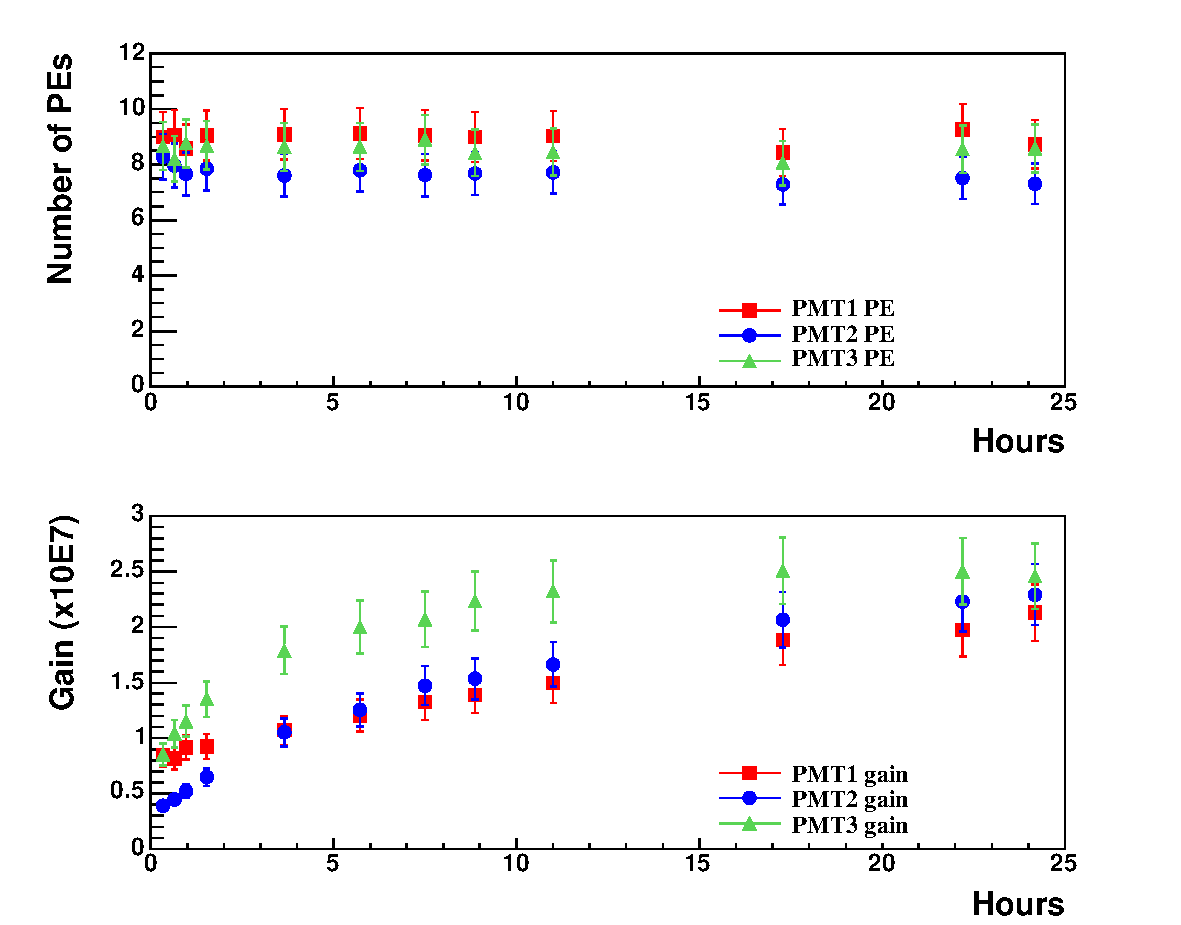
\includegraphics[width=0.75\textwidth]{RateDep1.pdf} 
%        \caption{The time dependence of the PMT gains with high rate LEDs (10 kHz)~\cite{Briese:2013wua}. As you see, the PMT gains take longer time to stabilize. }\label{fig:RateDep}
%\end{figure}


\subsubsection{Wavelength-Shifting Plates}
\label{sec:wavelengthshift}


In order to be sensitive to 128~nm VUV liquid argon scintillation photons, the optical assemblies use a wavelength-shifting coating to convert this VUV light to visible wavelengths that are detectable by PMTs.  In MicroBooNE, the active ingredient of this coating is TPB, an organic fluor which absorbs efficiently in the vacuum ultraviolet with an emission spectrum peaked around 425~nm \cite{Burton:1973} as shown in figure~\ref{fig:lightchallenge}. 

The optical unit PMTs observe light transmitted through TPB-coated, 12-inch diameter acrylic plates (see figure~\ref{fig:PlateCoating}).
The coating consists of a 1:1 TPB-to-polystyrene ratio, with 1 g of each dissolved in 50 ml of toluene.  A small amount of ethyl alcohol is added as a surfactant.
The coating is applied to the acrylic plate in three layers by brush-coating.  The solution dries in air at room temperature.
This leads to a final layer which is oversaturated with TPB, and white crystals form on the surface as the coating dries.  The presence of surface crystallization gives the MicroBooNE plates a white, opaque finish. Details of the process are described in reference~\cite{Ignarra:2014yqa}.

\begin{figure}[t]
\centering 
%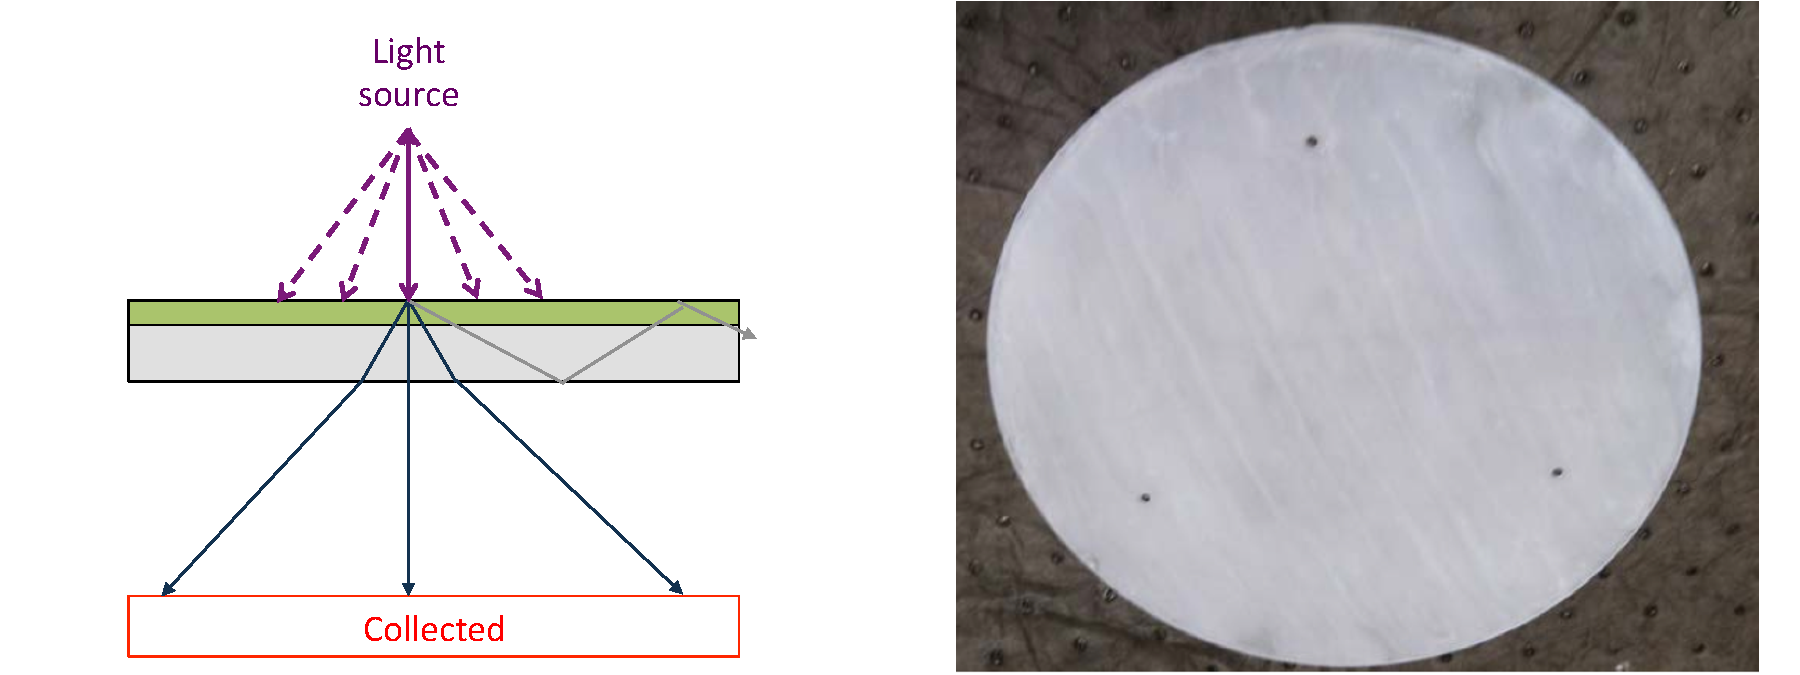
\includegraphics[width=\textwidth]{./light_figures/PlateModeAndPhoto.pdf}
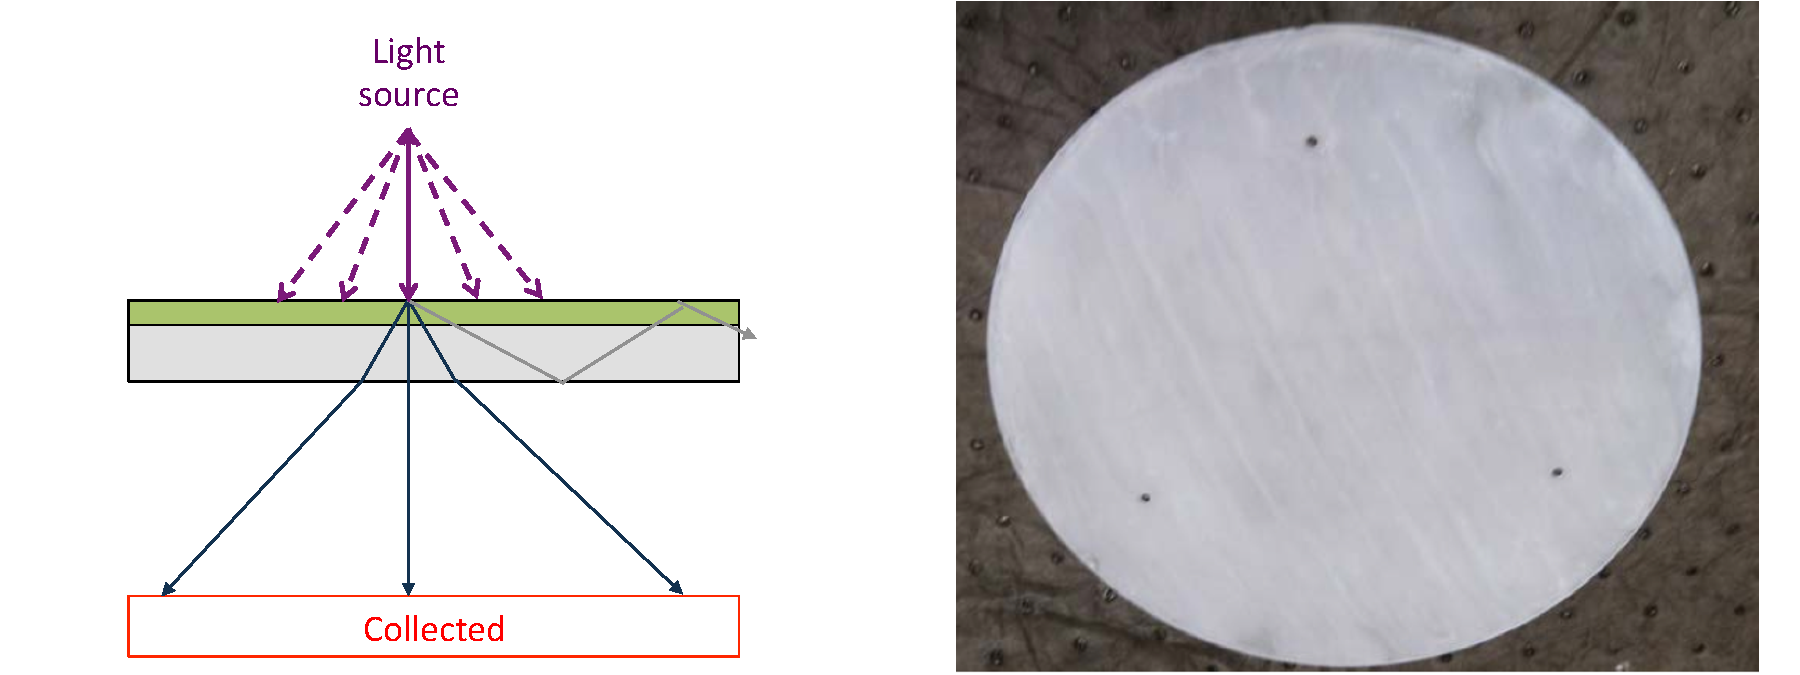
\includegraphics[width=\textwidth]{./light_figures/PlateModeAndPhoto.pdf}
\caption{Left : Illustration of transmission mode, used by the optical units. Right: photograph of a coated plate. \label{fig:PlateCoating}}
\end{figure}

The emission spectrum in figure \ref{fig:TPBSpectraPlate} was measured using a Hitachi F-4500 fluorescence spectrophotometer with an incident beam of wavelength 270 nm, selected by a diffraction grating from a xenon lamp.  A standard rhodamine dye calibration sample was used to correct for drift in the lamp and spectrometer.  The measurement was made in transmission mode, and an artifact peak at a harmonic of the twice incident wavelength was observed between 525 and 600 nm.  This region is omitted from the reported spectrum of figure \ref{fig:TPBSpectraPlate}.  

As shown in figure \ref{fig:TPBSpectraPlate}, although the absolute quantum efficiency for the platinum-undercoated cryogenic PMT is lower than the non-cryogenic version, the wavelength dependence is similar, and overlap between the TPB emission spectrum and the sensitive wavelength range of the PMT remains high.  Using the measured TPB emission spectrum for plate coatings and the PMT quantum efficiency curve provided, the spectrum-averaged PMT quantum efficiency is 15.3\% $\pm$ 0.8\% per visible photon incident on the photocathode. 

\begin{figure}[t]
\centering 
%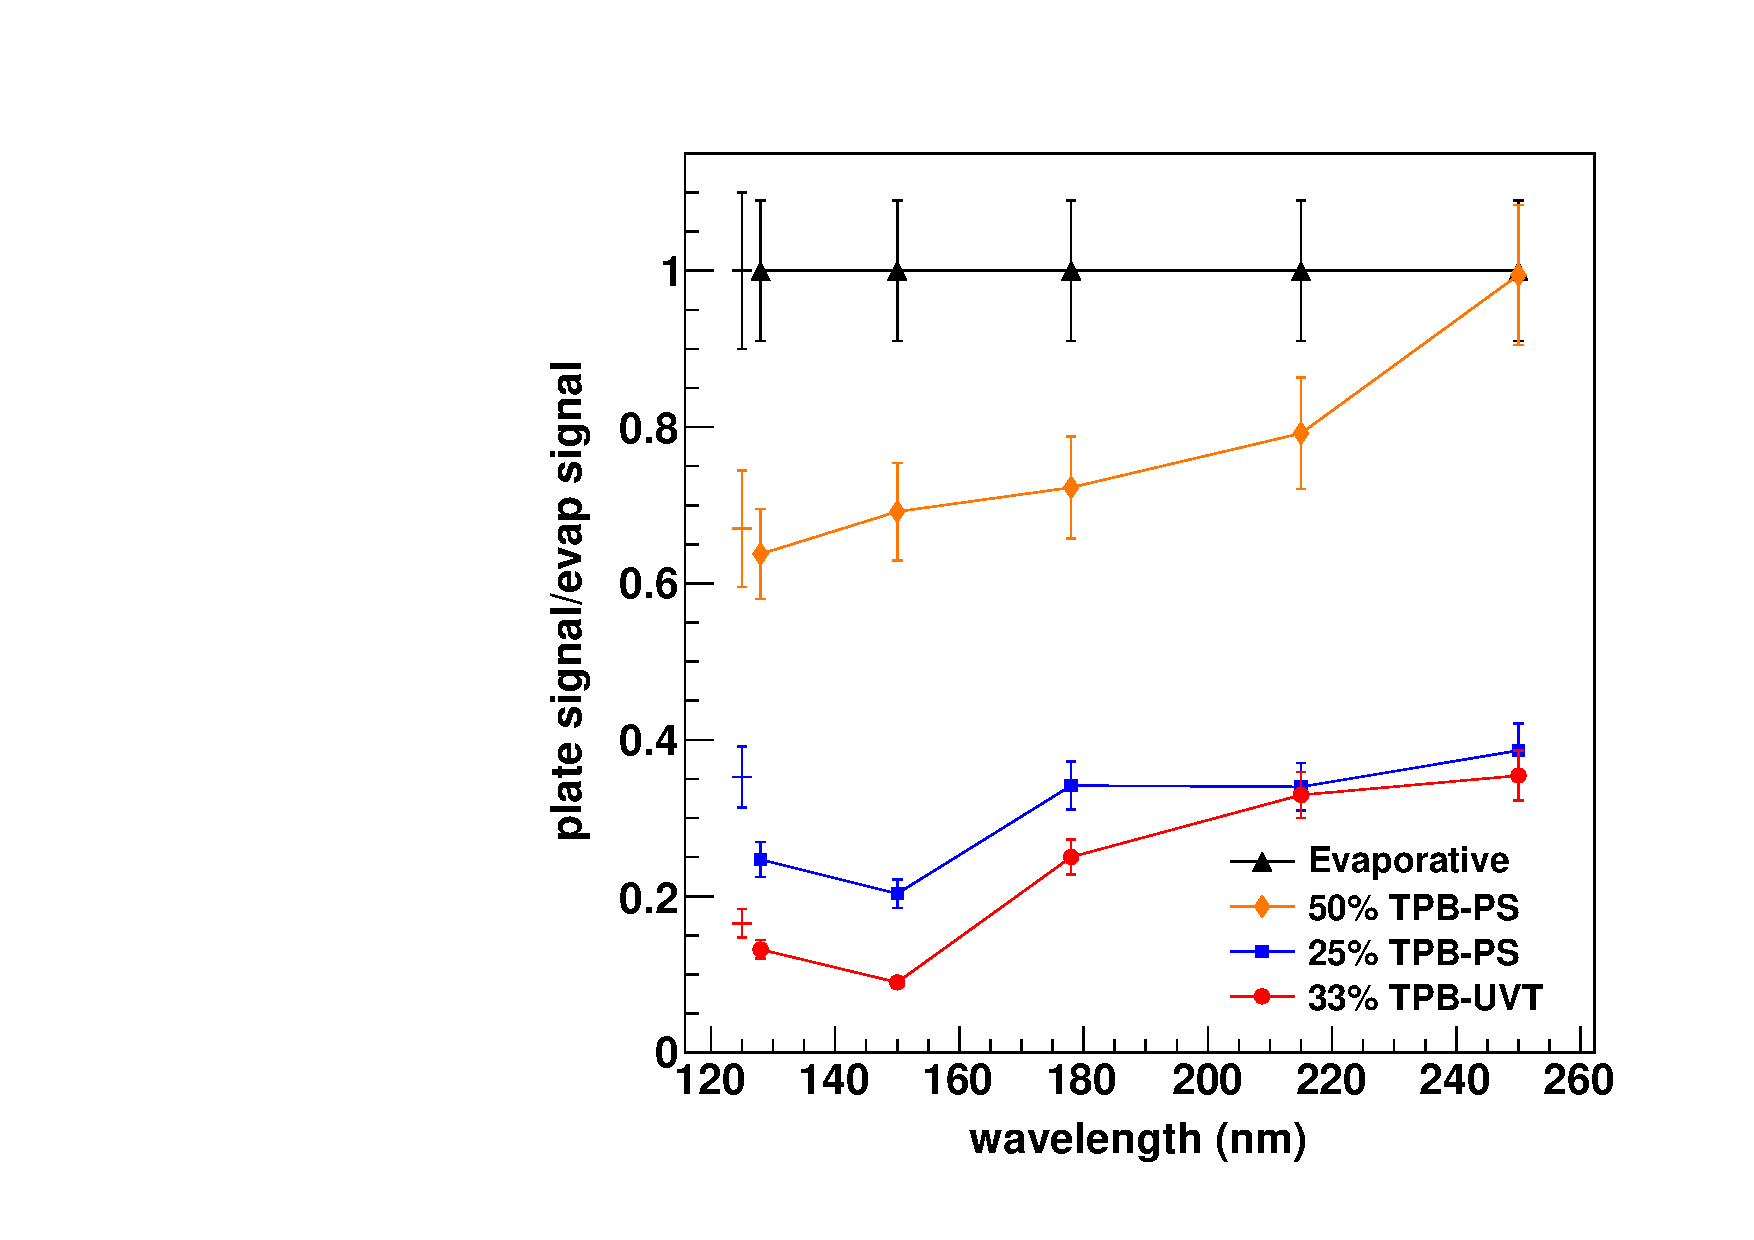
\includegraphics[width=0.6\textwidth]{./light_figures/EfficienciesIgnarraThesis.pdf}
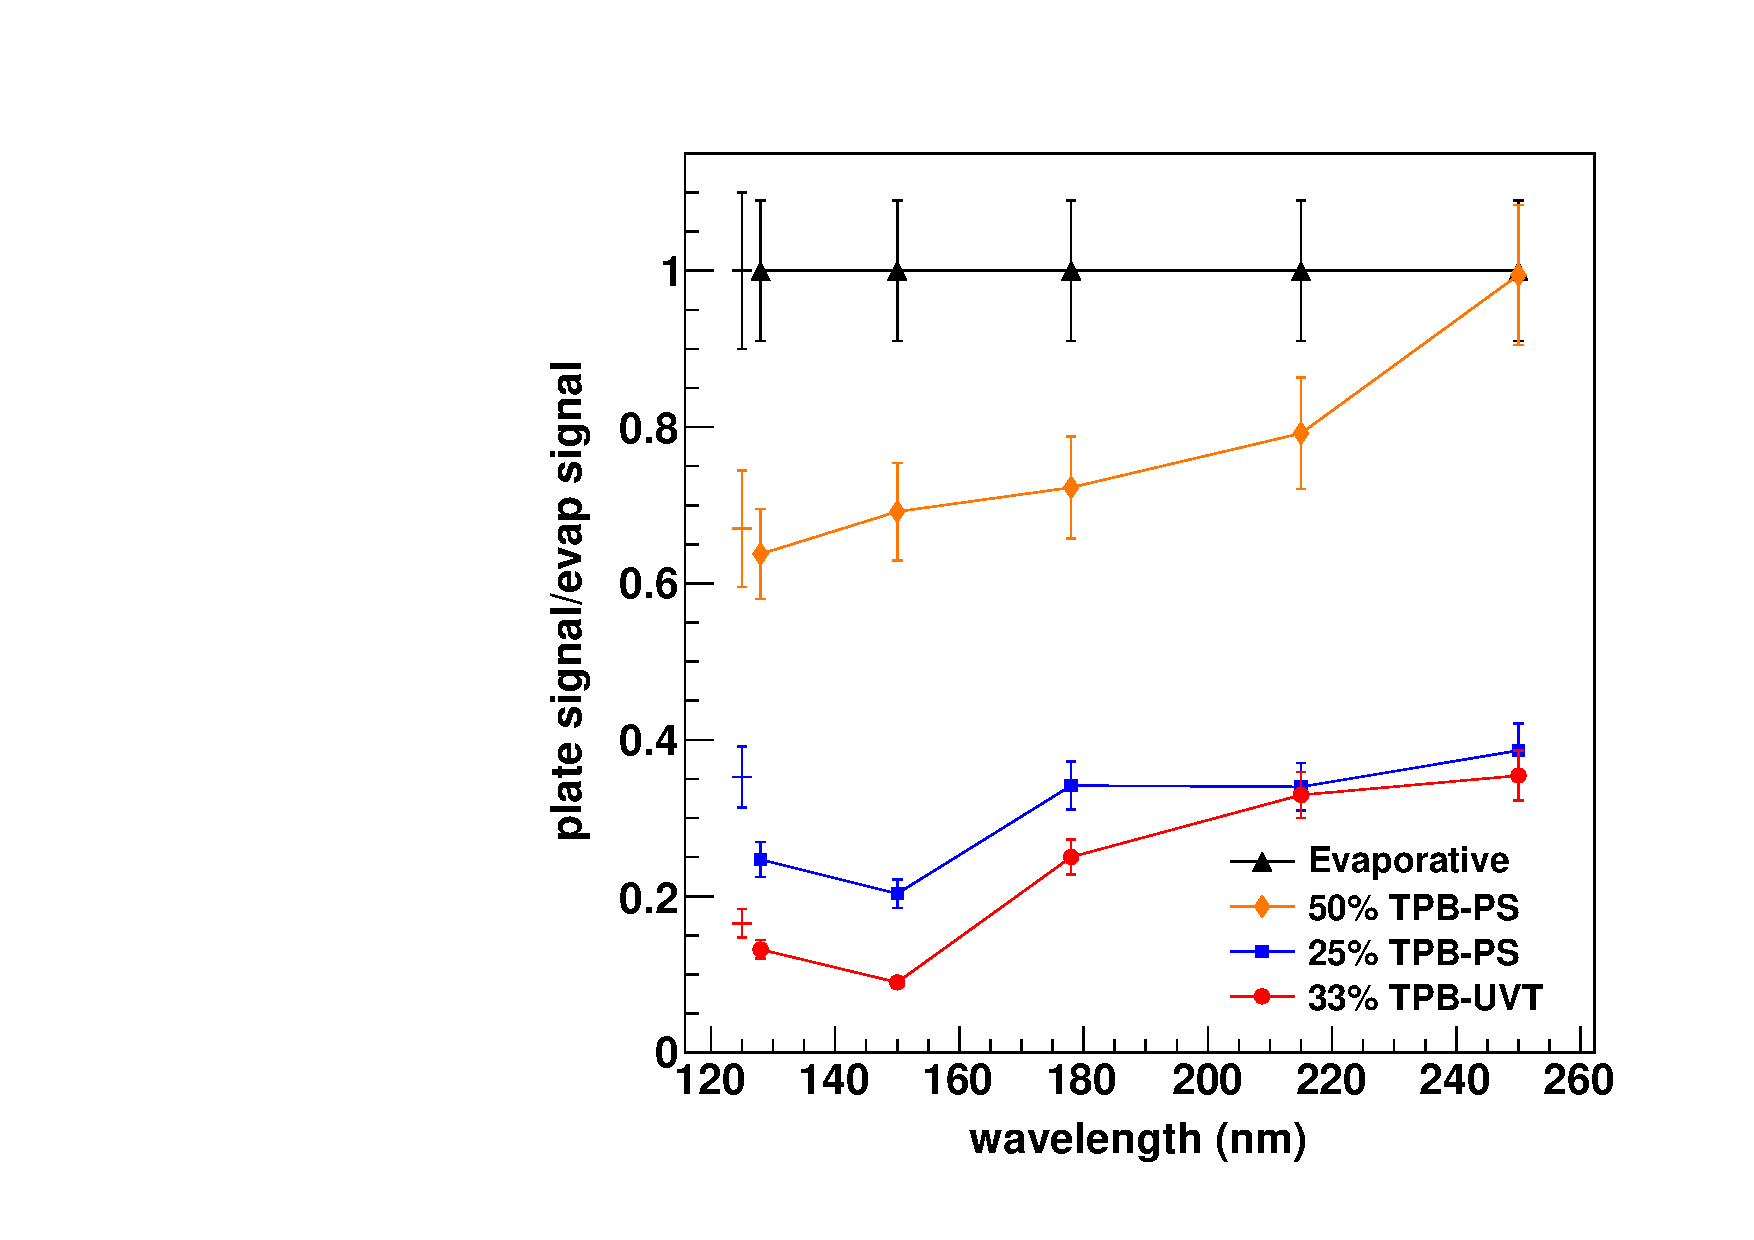
\includegraphics[width=0.6\textwidth]{./light_figures/EfficienciesIgnarraThesis.pdf}
\caption{Measured efficiencies of various wavelength-shifting coatings, from \cite{Ignarra:2014yqa}. In this plot, 50\%TPB-PS is the MicroBooNE plate coating used in the optical units.  The 33\%TPB-UVT is the light guide coating for the secondary light collection system described below.  Connected points were measured in a vacuum monochromator at room temperature, and non-connected points were measured in liquid argon with 128 nm scintillation light. All points are normalized to the performance of an evaporatively coated plate. \label{fig:CoatingEfficiency}  }
\end{figure}

The wavelength-shifting performance of the coating was measured at 128~nm relative to evaporative coatings of the type studied in \cite{Gehman:2011}.  Coating efficiencies were measured as a function of wavelength between 128 and 250~nm using a vacuum monochromator at room temperature.  They were also measured in liquid argon using 128 nm scintillation light, relative to the same evaporatively coated plate.  These data are shown in figure~\ref{fig:CoatingEfficiency}, and more information about these measurements can be found in \cite{Ignarra:2014yqa}.  
  
The absolute efficiency of the MicroBooNE coatings can be obtained by multiplying the relative efficiencies of figure \ref{fig:CoatingEfficiency} by the measured absolute efficiencies from \cite{Gehman:2011}, and accounting for the temperature dependence in the wavelength-shifting efficiency of pure TPB reported in \cite{Francini:2013-jinst}.  The expected efficiency of MicroBooNE coatings is found to be $0.98 \pm 0.17$ emitted visible photons per incident 128 nm photon for the plate coating.


\subsubsection{UV Light Protection for the Wavelength-Shifting Plates \label{environ}}

TPB coatings have been shown to degrade under exposure to ultraviolet light \cite{Chiu:2012} through a radical mediated photo-oxidation to the UV-blocker and photo-initiator benzophenone \cite{Jones:2013}.  Several measures were taken to ensure that degradation was minimized during the construction of the experiment.  The TPB powder and coated elements were stored in the dark at all times, with coated plates and light guides being kept wrapped in foil and stored in a dark container before installation.  The detector construction area was covered with a UV blocking plastic \cite{LexanThermoclear}, and test plates were placed at various positions in the clean tent to check for degradation from stray light.  After several weeks of exposure, one test plate with a clear line of sight to the tent entrance demonstrated a few percent degradation, and all others showed no observable loss of efficiency. The open end of the MicroBooNE cryostat was shielded from light by a black curtain after installation, and the feedthroughs of the cryostat were blocked when not in use to prevent stray light from entering.  The coated plates were the final component of the optical system to be installed into the detector to give the minimum possible light exposure during the detector construction process.

\subsubsection{Cryogenic Mu Metal Shields}

\begin{figure}[t]
\centering 
%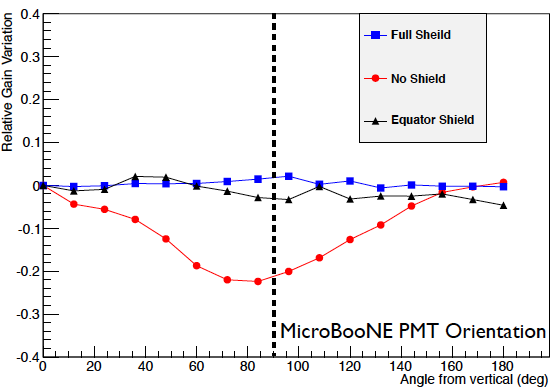
\includegraphics[width=0.6\textwidth]{./light_figures/shield.png}
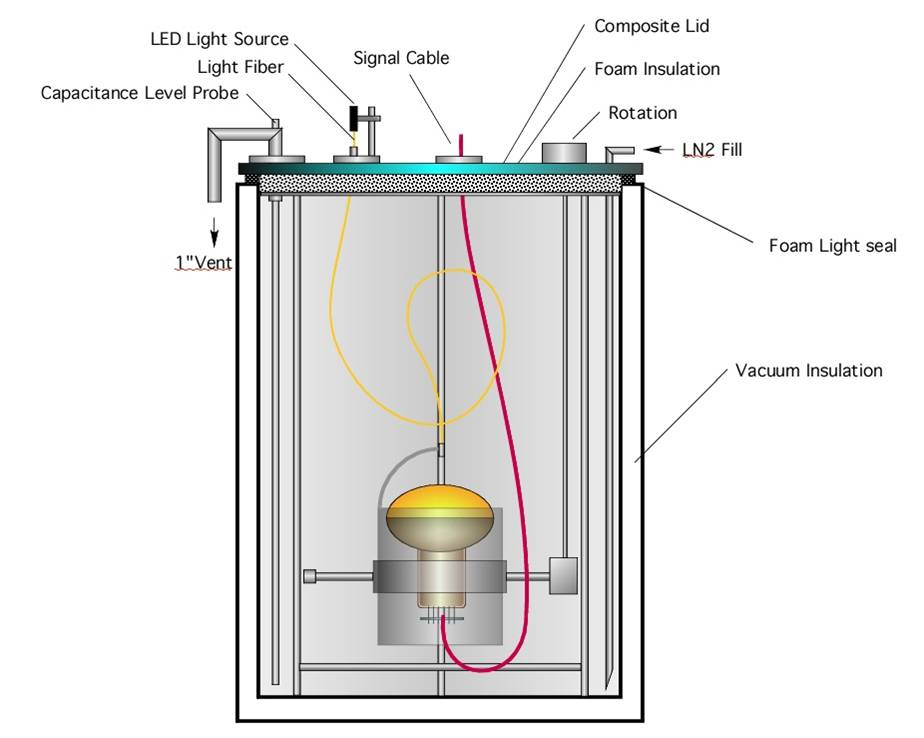
\includegraphics[width=0.8\textwidth]{./light_figures/KendzioraRotator.jpg}
\caption{Schematic of the system used to study the mu-metal shields.  The design allows rotation along all three axes. \label{fig:shieldcartoon}  }
\end{figure}



\begin{figure}[t]
\centering 
%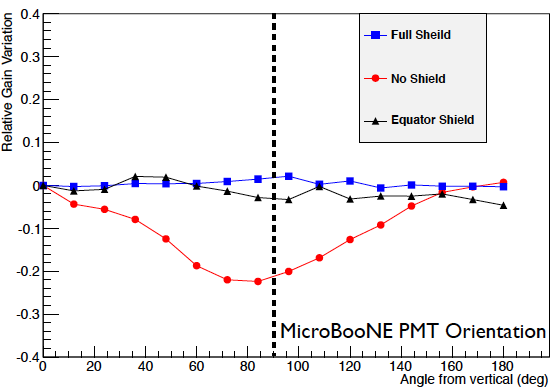
\includegraphics[width=0.6\textwidth]{./light_figures/shield.png}
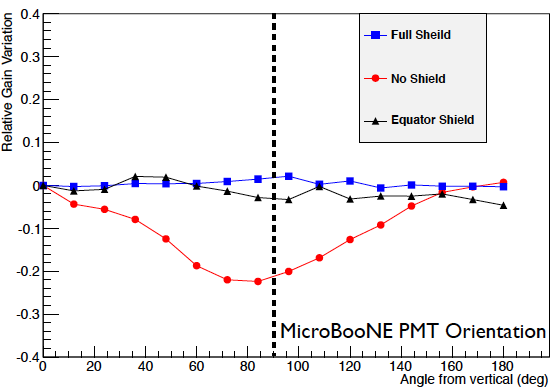
\includegraphics[width=0.6\textwidth]{./light_figures/shield.png}
\caption{Red:  Angular dependence of a PMT response with no shield;  Black:  for a shield that reaches the tube equator;  Blue: for a shield that fully covers the tube to the zenith. \label{fig:shield}  }
\end{figure}


%{\bf The following text is from  http://microboone-docdb.fnal.gov:8080/cgi-bin/ShowDocument?docid=2085 and  http://microboone-docdb.fnal.gov:8080/cgi-bin/ShowDocument?docid=2159}

The trajectories of electrons within the 8" PMT can be deflected by the Earth's magnetic field.  This effect can be reduced or removed by surrounding the PMT with mu metal, a metal of low magnetic permeability.  Commonly used mu-metal fails to provide shielding at cryogenic temperatures. Two types of cryogenic mu metal, Cryoperm 10 and A4K, both products of Amuneal, were identified that did provide shielding at cryogenic temperature. 

The mu metal shields were tested in the apparatus shown in figure~\ref{fig:shieldcartoon}.  The system allowed for the PMT to be positioned at an angle relative to the vertical axis, with the rotator set to 30 positions from 0 to 348$^\circ$.    The set-up was on a dolly that allowed for rotation about the vertical axis.  PMT tests were performed in air and in liquid nitrogen.   PMTs were dark adapted for 5 hours before testing.  %Each data run consisted of a single dolly position and 30 angles from vertical, and took about four hours to complete.
A blue LED provided 1 to 2 single PEs of light through an optical fiber.   The fiber was fixed to the PMT mount such that the endpoint was stationary with respect to the tube as the system was rotated.   

The mean charge from the PMT as a function of angle was recorded.  The error was primarily systematic.   The $\sim10^6$ to LED pulses per data point give $<1\%$ statistical error on the mean.  However, 24-hour studies of a single point showed $\sim5\%$ variations in collected charge due to gain drift.  Results showed that A4K and Cryoperm function essentially identically, to within the measurement error, and so MicroBooNE chose A4K, based on significant cost savings.    A plot of the relative PMT gain variation versus angle from vertical, figure~\ref{fig:shield}, shows that adding the shield significantly improves PMT performance.  This plot shows the effect of the A4K shield with the height aligned with the equator of of the PMT (black) and aligned with the zenith of the bulb (blue), compared to no shield (red) as a function of PMT azimuthal angle.  Given the 5\% systematic error, the two shield positions are indistinguishable.  

As a result of these tests, the A4K shields were designed to extend just past the equator of the PMT.  The shield has small holes in the backplate that allows the PMT cables to exit the shield.   MicroBooNE is the first \lartpc to use cryogenic mu metal shields in its light collection system.  


\subsubsection{Implementation of the Primary System \label{LCUnitimplement}}

%This section describes the implementation of the light collection system.  Specifically, description is provided for the unit assembly, rack mounting of units, cable system, feedthroughs, an AC-coupling circuit referred to as the "splitter", and high voltage supplies.

The light collection system is composed of optical units assembled as shown in the top picture of figure~\ref{fig:unitmodel}.  The PMT is seated within the mu metal shield on three teflon pads attached to an equatorial support ring.  The neck of the tube slides inside a loose wire guide-loop that prevents the PMT from tipping.  The PMT is held within this assembly using teflon-encased wires that extend across the bulb and connect to wire hooks attached to the equatorial ring with stainless steel springs. Legs extending from the support at the equator are screwed into a backplate for final mounting.  Concern about differences in contraction of the materials led to this design which holds the PMT in place, but with only moderate rigidity.  The units were tested to ensure the PMTs would not be displaced during installation and filling.  Three posts extend upward from the equatorial ring to hold the plate 3.0 cm above the apex of the bulb.   The optical units slide into a cylindrical mu-metal shield, which screws into the equatorial ring.  The unit is then mounted on stainless steel back-plates affixed to a support rack, as shown in the bottom picture of figure~\ref{fig:unitmodel}.

\begin{figure}[t]
\centering	
%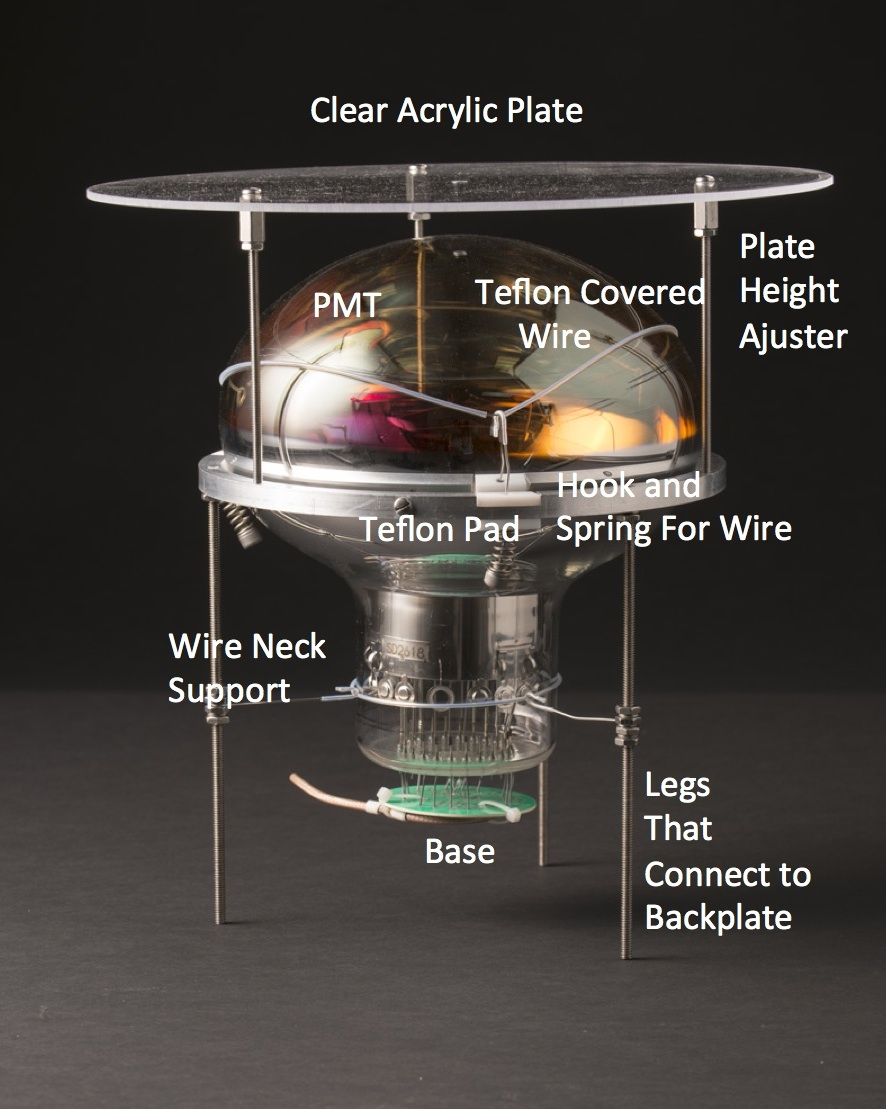
\includegraphics[width=0.45\textwidth]{./light_figures/mountedpmtlabeled.jpg}
%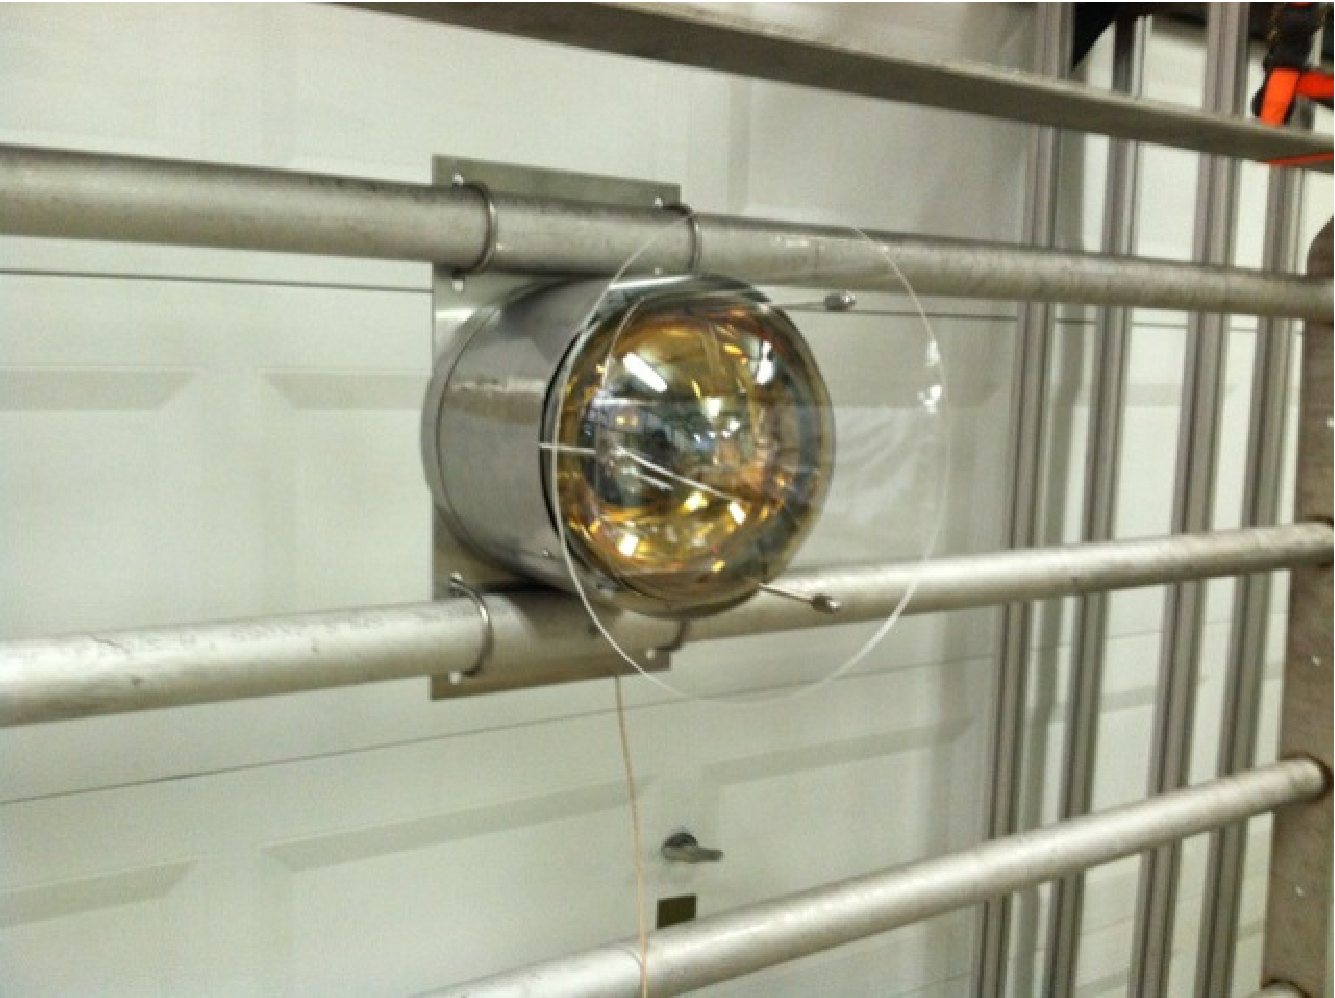
\includegraphics[width=0.45\textwidth]{./light_figures/PMTunit2.pdf}
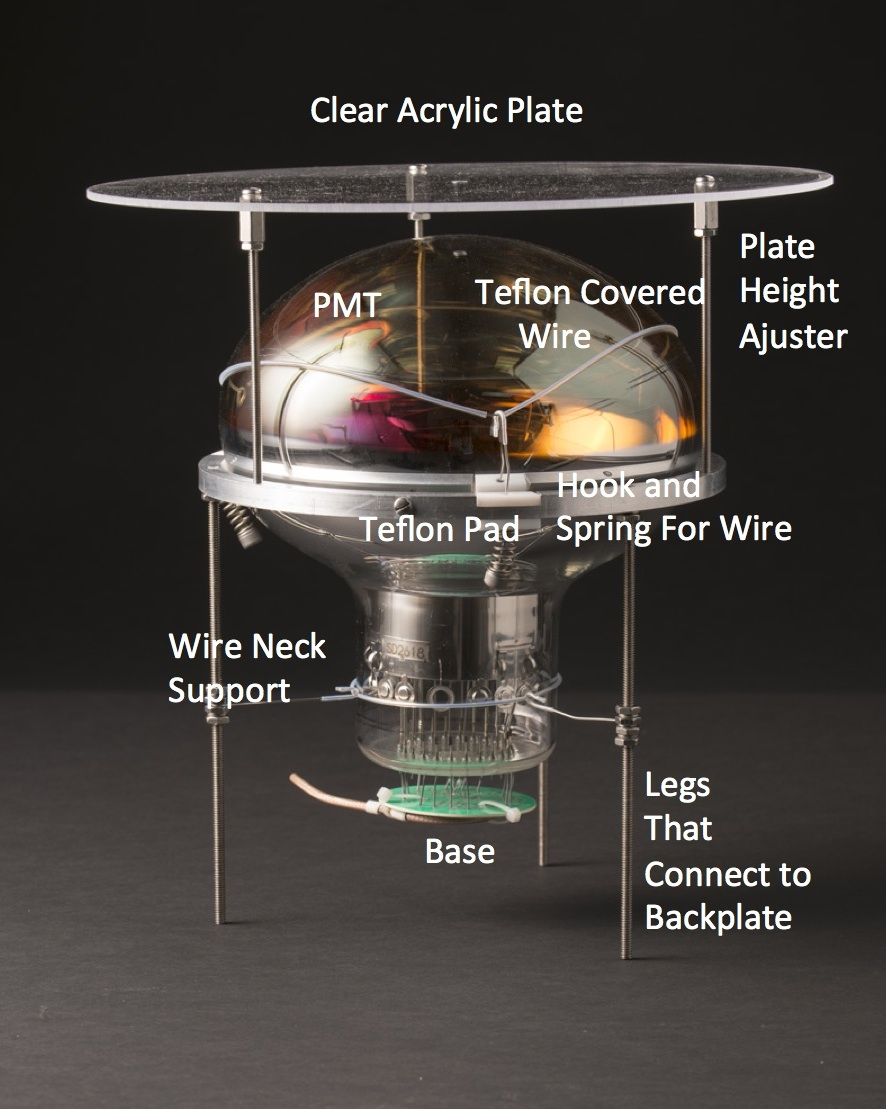
\includegraphics[width=0.65\textwidth]{./light_figures/mountedpmtlabeled.jpg}
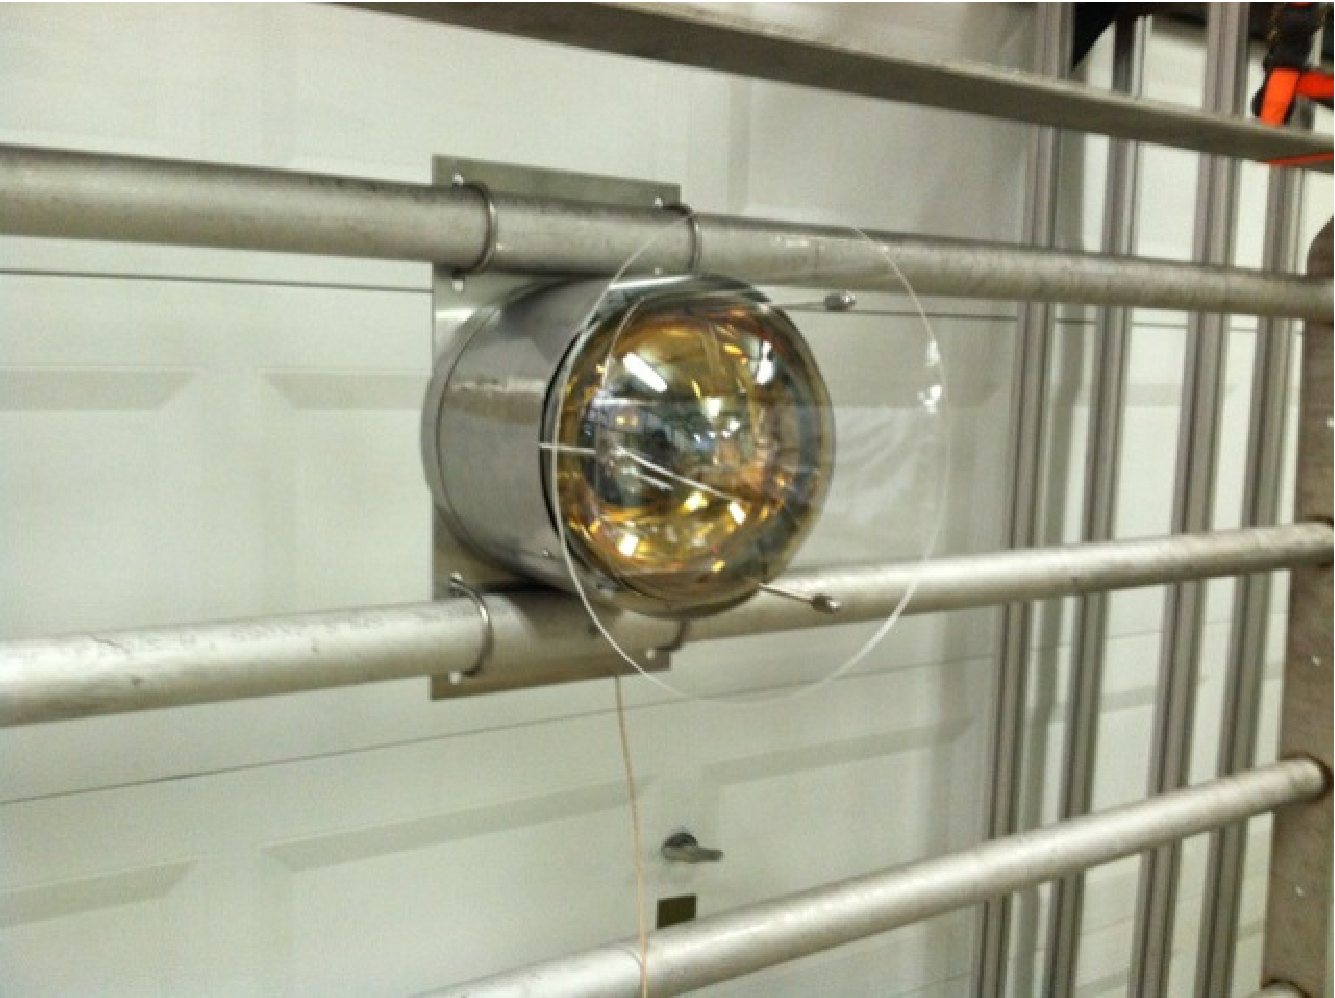
\includegraphics[width=0.65\textwidth]{./light_figures/PMTunit2.pdf}
\caption{Top The optical unit mount internal to the shield, with components labeled; Bottom: Unit mounted on rails.  The clear plates were replaced with TPB-coated plates immediately before \lartpc installation, as discussed in the text~\cite{Briese:2013wua,Katori:2013wqa}.}
\label{fig:unitmodel}
\end{figure}

The support rack consists of five stainless steel components, or modules, for ease of installation.  Each module has vertical height 1.83 m and horizontal length 2.07 m, resulting in a total horizontal length of 10.36 m.  Unlubricated Thomson bearings fitted to the lower edge allow each module to slide into the cryostat on rails mounted in the vessel.   The system was designed to allow the light detection system to slide into the vessel after the \lartpc was installed.  However, in the end, scheduling permitted installation of the system before the \lartpc installation.  This had the advantage of making installation and surveying easier, but the drawback that the system would be exposed to UV light for a long period.  Therefore, the units were installed with dummy clear acrylic plates, and the TPB coated plates were installed only just before the \lartpc was moved in and the detector could be easily protected from light.  During optical unit installation, each rack module was supported by a temporary mounting rail.  The optical units were then mounted in positions chosen to avoid obstruction by the \lartpc cross-bars, as shown in figure~\ref{fig:lightlayout}.  As the units were mounted and slid into the cryostat, the cables were loosely tied to the bars of the rack for support and constraint.  

The ``splitter'' circuit, located outside of the cryostat, is shown in figure~\ref{fig:splitter}. The splitter separates the HV of the PMT from its output signal which is subsequently split into a high-gain (HG) and a low-gain (LG) channel. The HG and LG channels respectively carry 18$\%$ and 1.8$\%$ of the output signal.  This allows a wide dynamic range for ADC readout of the PMT pulses.  The capacitance was chosen to minimize reflections, since the bases are not back-terminated.  The HV is supplied to the splitter using BiRa Corporation, Model 4877PS modules.

\begin{figure}[h]
\centering 
%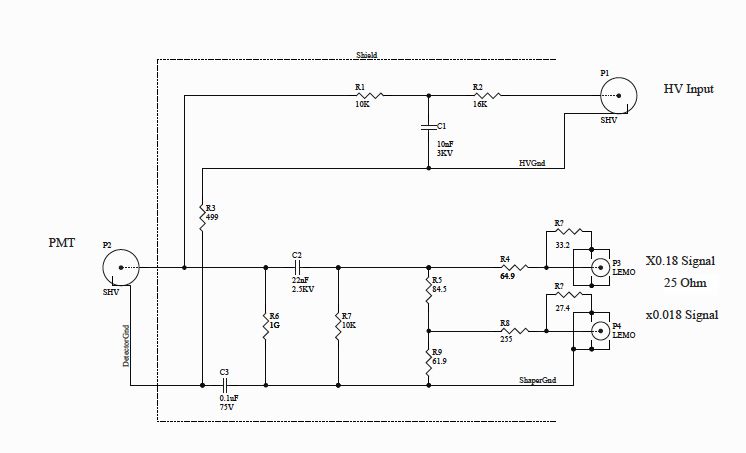
\includegraphics[width=0.7\textwidth]{./light_figures/splitter.png}
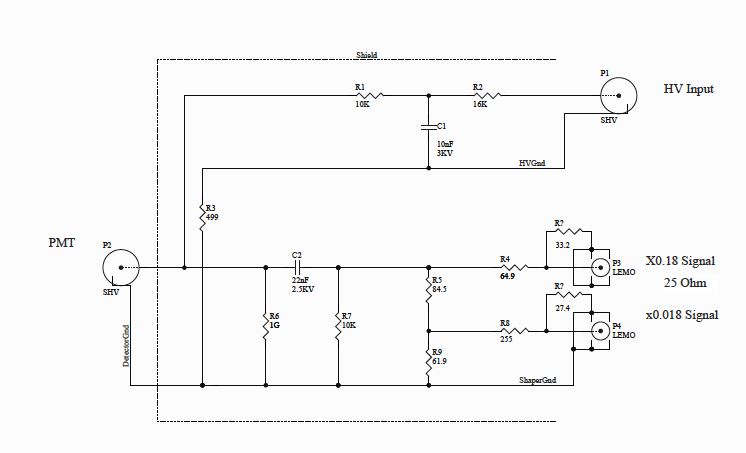
\includegraphics[width=0.7\textwidth]{./light_figures/splitter_modified.png}
\caption{The ``splitter'' circuit.  The circuit connects the HV source to the PMT. It also provides a pathway for signal pulses from the PMT to reach the readout electronics via an AC-coupling capaciter (C2).  The signal is split into two copies, one provided with an attenuation factor of 0.18 and another at 0.018. Both signal sources are recorded by the readout electronics in order to provide two dynamic ranges.}
\label{fig:splitter}
\end{figure}


The PMT cable system delivers HV and returns signals between the external splitter and the optical unit in the cryostat.   A single cable runs from an external connector, through the feedthrough filled with Stycast 2850 epoxy \cite{stycast}, into the cryostat and to the PMT base. The RG316/U coaxial cable has 50 Ohm impedance.  Cables were terminated with Pasternack PE4498 SHV to accommodate that the cable carries HV to the tube as well as signals from the tube.
%0.36 cm diameter cable has 95 ohm impedance to match with the pre-amplifier and low capacitance of 6.8 pF/m to preserve small signals.  
The cable carries an AC voltage rating of 1100 V; however tests showed the DC rating to be at least three times higher and so suitable for this use.  The cables were routed through feedthroughs consisting of a pipe filled with solidified epoxy mounted on a conflat disk.  On the warm side of the feedthrough, the cables were terminated at a patch panel with SHV connectors. The SHV connector impedance has a negligible effect on the 20-30 ns PMT signals.  SHV cables connect the patch panels to the splitters.  The impedance of every channel was tested at the feedthrough patch panel for a stable and correct value for the base resistance, which was 4.04$\pm$0.02 M$\Omega$ for the 8-inch PMTs. 

\subsection{PMT Testing and Quality Assurance}

\begin{figure}[t]
\centering 
%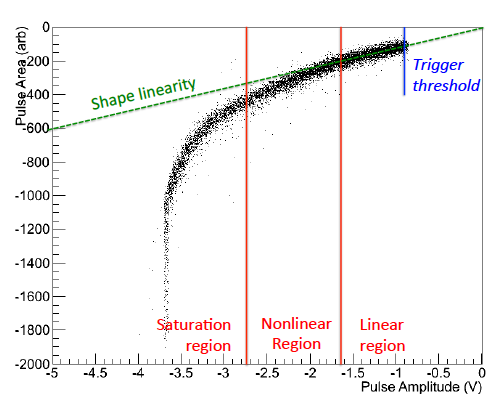
\includegraphics[width=0.9\textwidth]{./light_figures/nonlinear.png}
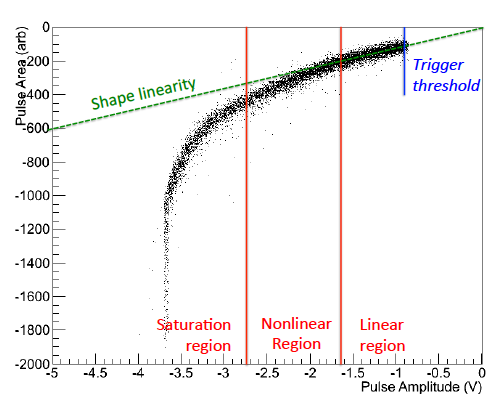
\includegraphics[width=0.9\textwidth]{./light_figures/nonlinear.png}
\caption{\footnotesize As shown by the VST, linearity of cosmic-ray induced PMT pulses is maintained up to amplitudes of around 1.7 V (300 PE), and amplitude saturation occurs at 3.7 V (670 PE) \cite{Jones:2015bya}
 \label{fig:nonlinear}  }
\end{figure}

The PMTs were tested and characterized before installation in the detector in the ``Bo'' cryostat at Fermilab.  The Bo cryostat is a 250-liter vacuum-insulated vessel with an inner diameter 22 inches and a depth of 40 inches used for R\&D studies, and, relevant to this paper, a vertical slice test of the MicroBooNE optical units.  The system is described in detail in reference~\cite{Jones:2015bya}.  The cryostat can be filled with purified LAr with parts per billion level contamination of oxygen and water and parts per million level of nitrogen.  The light collection system was tested with light from visible (420 nm) and UV (250 nm) LEDs piped in via fiber, as well as scintillation light from $^{210}$Po alpha sources and cosmic rays.

A vertical slice test (VST) of the MicroBooNE optical system was performed in the Bo Cryostat.  The slice consisted of two 8 inch PMTs with base electronics, mu-metal shield, TPB plates,  cable feed throughs, splitters, the HV power supply and the interlock system.   Tests were performed without and with the mu-metal shield.   The test made use of the DAQ components described in section~\ref{sec:electronics}, including the shaper, FEM, trigger card, control card, and server.  The MicroBooNE trace impurity monitors were also used.

The VST informed the final design of many components, as well as producing results relevant to understanding the running conditions and performance expectations.   For example, during studies of the response of the slice to 128 nm scintillation light from the alpha source, 
valuable information was gathered on the single photo-electron dark rate and cosmic ray rate that could be scaled to the MicroBooNE detector expectations.    As a second example, these runs allowed characterization of the pulse shape nonlinearities of the optical units, as seen in figure~\ref{fig:nonlinear}.  These were shown to be significant at $\sim$300 photo-electron in pulse amplitude.  Full amplitude saturation occurred at $\sim$670 PE. Thus, it is concluded that for pulses of more than 300 PE, pulse shape cannot be described by linear superposition of single photoelectron pulses. 


\subsection{Secondary System: Acrylic Light Guides for R\&D}


\begin{figure}[t]
\centering 
%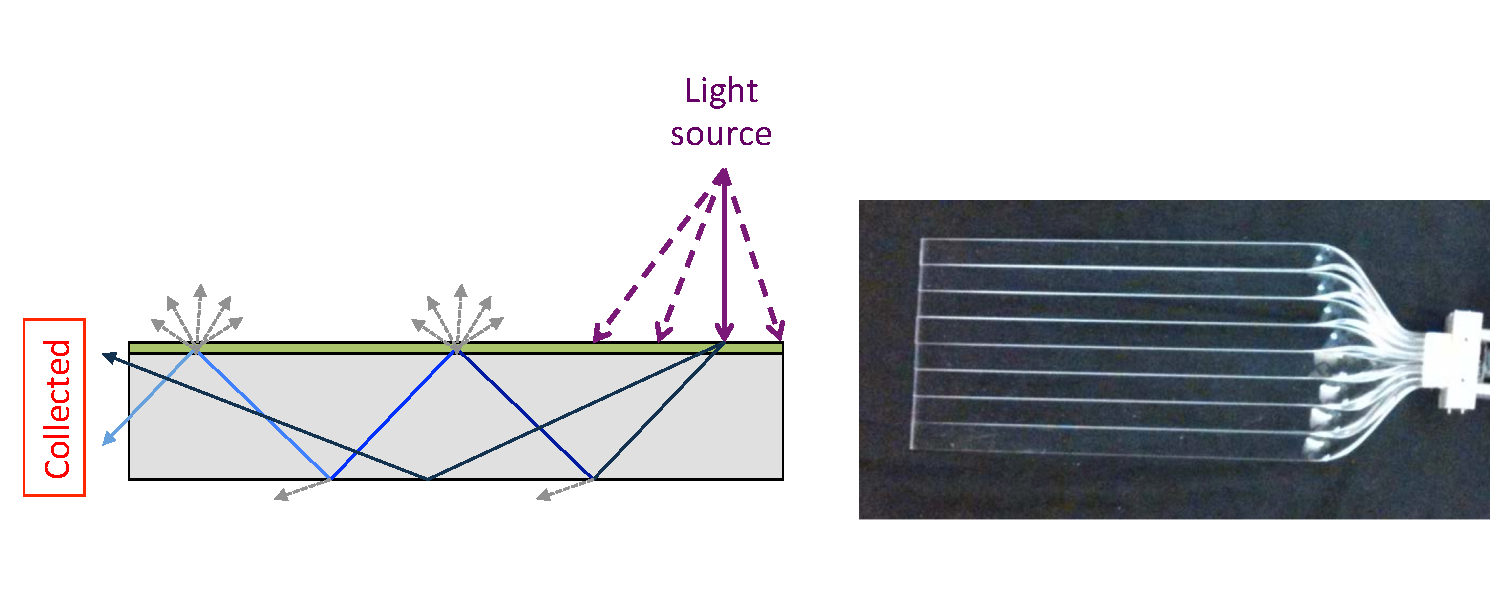
\includegraphics[width=\textwidth]{./light_figures/LightguideModeAndPhoto.pdf}
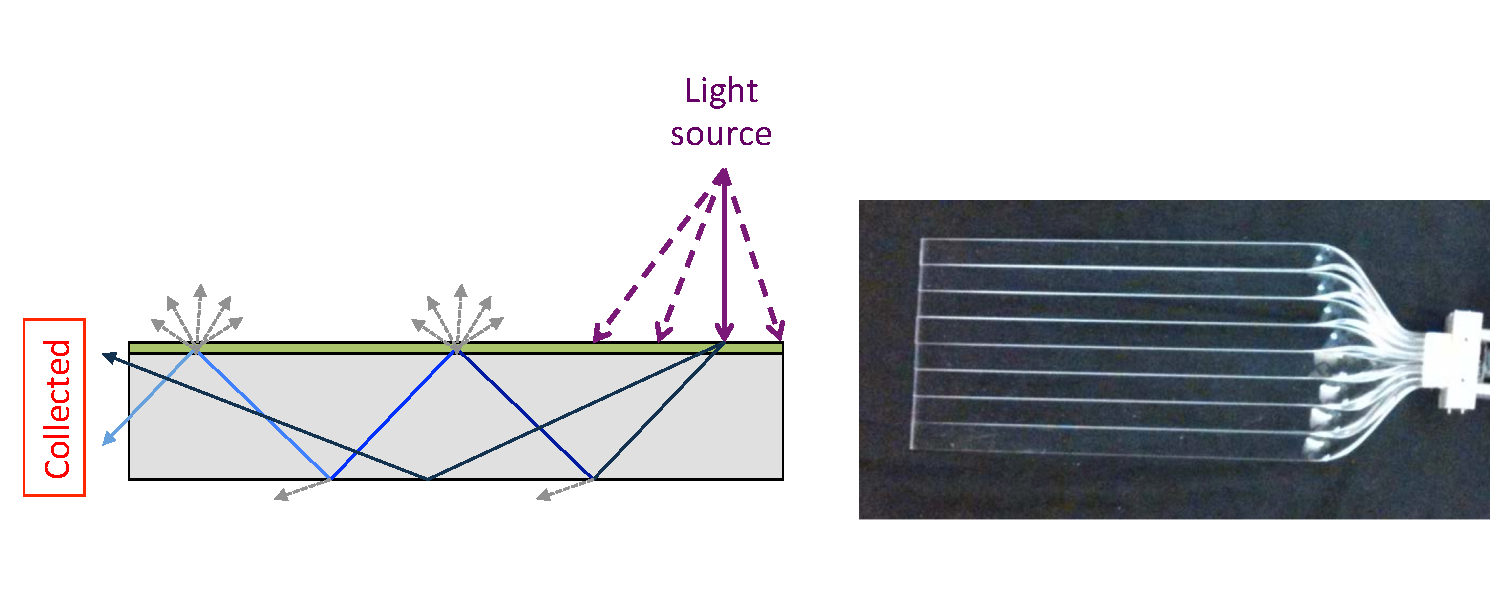
\includegraphics[width=\textwidth]{./light_figures/LightguideModeAndPhoto.pdf}
\caption{Left : Illustration of guiding mode, used by the paddles. Right: photograph of a coated paddle. \label{fig:LGCoating}}
\end{figure}


A secondary light collection system consisting of four lightguide paddles was also installed.   This concept has several advantages for future large detectors such as DUNE. First, the collection area per channel is larger than the optical units, providing more coverage for the same number of electronics channels, cables, and feedthroughs.  Second, the detectors have a flat profile so they can be slid between chambers in a multi-\lartpc detector, minimizing space requirements of the light collection system.  In the case of MicroBooNE, the design gradually guides light in bent acrylic bars to a PMT.  This design was an early alternative to a perfectly flat design that guides the lights to SiPMs.  Running this system will provide long-term information on performance of lightguide based systems.  It also enhances the MicroBooNE dynamic range, since the lightguide detectors saturate at a much higher light level than the optical units.

In the case of the lightguides, the 128 nm light is absorbed and shifted by a clear wavelength-shifting coating, and the re-emitted light is guided to a 2-inch Hamamatsu R7725-MOD PMT, as illustrated in figure~\ref{fig:LGCoating}, left. The installed paddles consist of six bars.  A photograph of one coated paddle with eight bars is shown in figure~\ref{fig:LGCoating}, right.  The active length of each bar is 20 inches.  This system was added for R\&D purposes and made use of 8 spare channels available of HV, cables, feedthroughs, and electronics.  The impedance of the 2 inch PMTs, tested at the feedthrough, was 4.89$\pm$0.01 M$\Omega$.  As shown in figure~\ref{fig:lightlayout}, each paddle is installed next to an optical unit for direct comparison of performance.

The coating requirements for plate assemblies and light guides are different, and so the composition and coating methods for each were separately optimized.    In the case of the light guide coatings, the figure of merit is the light emitted in guided mode.  Guided mode light is the light that is detected at one of the ends of a test sample, which is orthogonal to the illuminated face of the sample.  In addition to the wavelength-shifting efficiency of the active layer, the detected light yield is affected by the reabsorpative and scattering losses in the coating as visible light propagates along the bar. The light guide assemblies have a TPB coating of 33\% TPB to 67\% UVT acrylic by mass, also with ethanol surfactant. The coating is applied as a single layer and the TPB remains suspended in the acrylic matrix as the coating dries, leading to a smooth, visibly transparent surface.  The performance and attenuation behavior of similar light guides to those installed in MicroBooNE were studied experimentally in \cite{Baptista:2012}.  The reported non-exponential attenuation suggests that surface losses dominate over bulk losses as the attenuation mechanism, and that the fractional loss per reflection within the light guide is of order 2-3\% \cite{Jones:2013}. 

In the light guide coatings, the TPB is suspended in an acrylic matrix which leads to a slight broadening of the emission spectrum compared to the spectrum from the plates. This is an expected effect--TPB fluorescence has been shown to have dependence upon its microenvironment \cite{Birks:1959,Birks:1961,Francini:2013-jinst,Hanagodimath:2008, Liu:1997}, and reference~\cite{Francini:2013-jinst} demonstrated spectral broadening in the presence of a polystyrene substrate.  Using the monochromater described for the plate spectrum studies, the light guide coating spectrum was measured in guided mode. A 10 cm section of light guide, with the incident beam perpendicular to the TPB coated surface, was used.  Based on reference \cite{Francini:2013-jinst} it is expected that the emission spectrum for the light guide coating, with TPB embedded in the substrate, will not change significantly as it cools to 87 K.  The expected efficiency for the light guide coating is found to be $0.25 \pm 0.05$ emitted visible photons per incident 128~nm photon.

\begin{figure}[t]
\centering 
%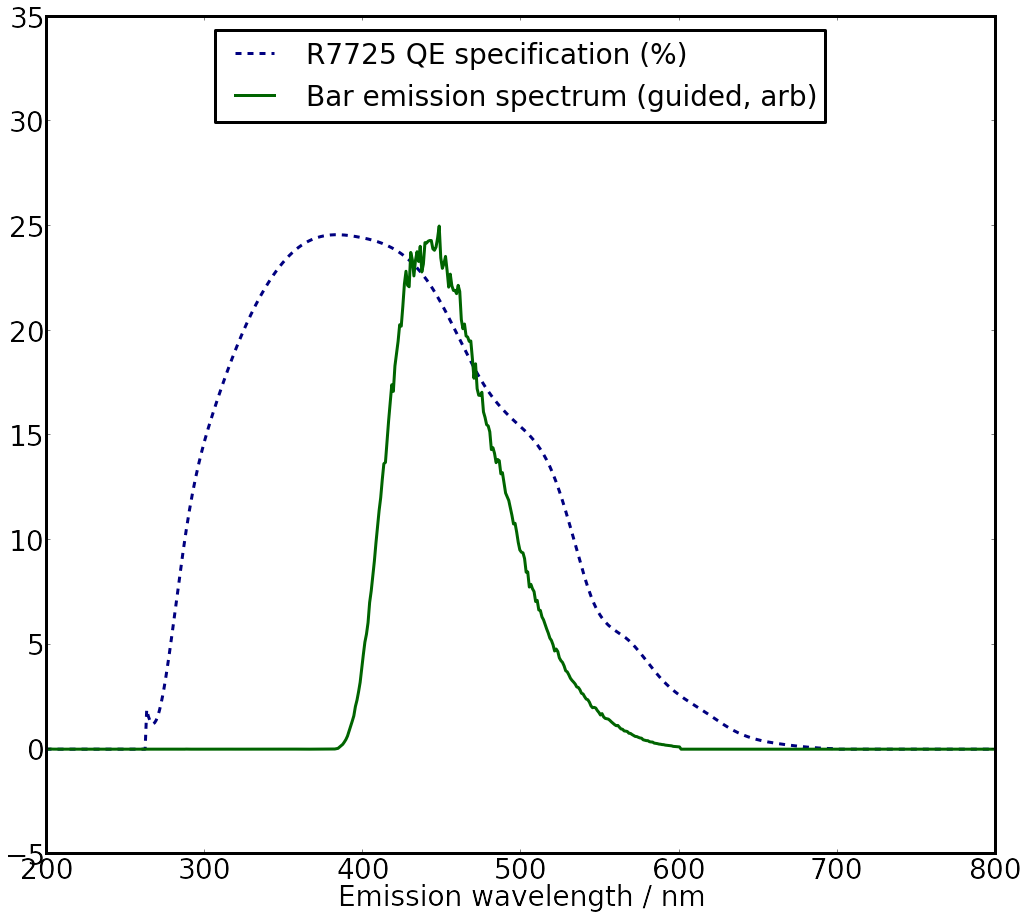
\includegraphics[width=0.65\textwidth]{./light_figures/BarSpectra.png}
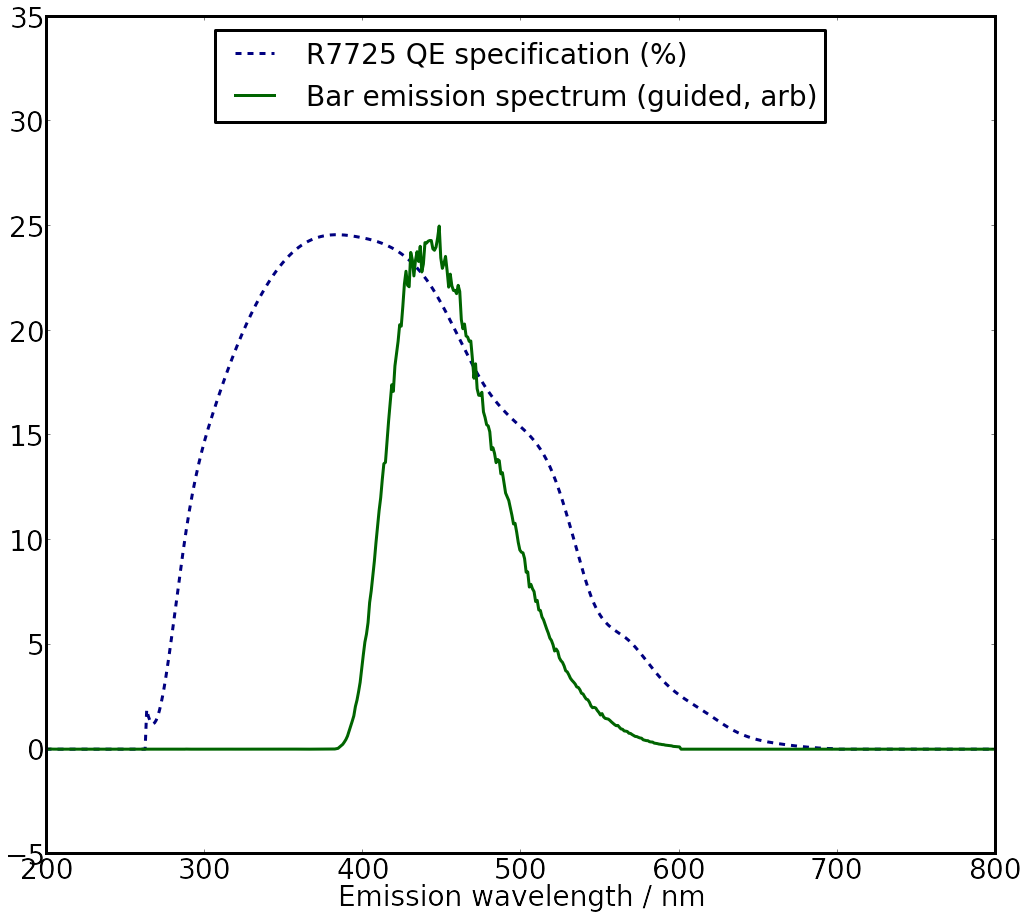
\includegraphics[width=0.65\textwidth]{./light_figures/BarSpectra.png}
\caption{Measured emission spectra of the light guide coating in guided mode, and the R7725 quantum efficiency.  Only the quantum efficiency of the non-undercoated PMT model is shown, from \cite{Hamamatsu-Datasheet2inch}.
 \label{fig:TPBSpectra}  }
\end{figure}

\subsection{Calibration}

The flasher system for the optical units and the light guides is described in reference~\cite{Conrad:2015xta}. This system was developed to check the timing of the installed optical units, exercise the optical units during construction and commissioning, and to calibrate them once the detector is operational.  The reference provides engineering drawings and details.  The system is briefly summarized here.

A control board pulses an array of 400 nm LEDs, each of which is
coupled through an optical feedthrough to 10 m optical fibers within the cryostat.  The custom feedthrough/patch panel design encases the fibers in Arathane CW 5620 blue with HY 5610 hardener.  The internal fibers are Molex FVP polymide fibers with diameter of 600 mm, cladding of 30 $\mu$m, and an additional buffer layer of 25 $\mu$m.  Each PMT has an individual calibration fiber.  Each fiber is routed along the rack  and attached to the PMTs by a fiber holder constructed of an aluminum standoff with a nylon-tipped set screw at a distance of about 2 inches from the PMT glass.

Figure~\ref{fig:flasherresult} shows the results of flasher tests on all 32 optical units and four PMTs on the paddles.  Time is along the $x$ axis and PMT channel number is along the $y$ axis.  The white region separating the optical unit PMTs from the paddle PMTs represents unused channels.  The colored bars indicate charge detected in the PMTs during flashing.  One can see that all tubes respond properly.


\begin{figure}[t]
\centering 
%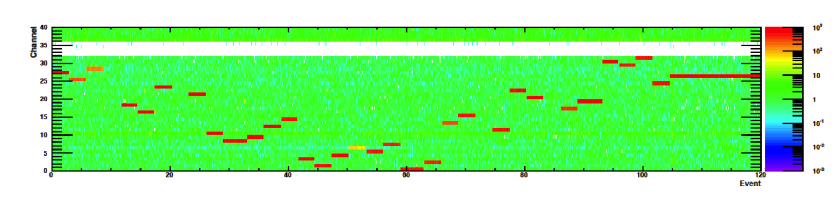
\includegraphics[width=\textwidth]{./light_figures/flasherresult.png}
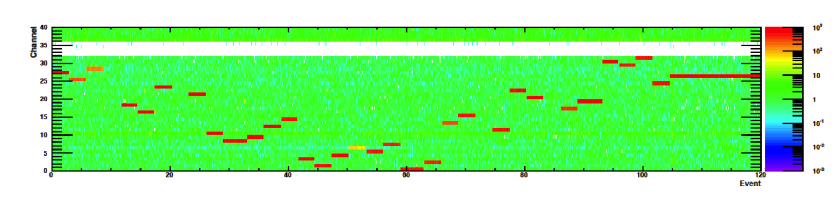
\includegraphics[width=\textwidth]{./light_figures/flasherresult.png}
\caption{Charge detected in each PMT due to flasher tests, shown as a function of time.  Each PMT is flashed for a short period. The white band indicates unused channels. \label{fig:flasherresult}  }
\end{figure}



\subsection{Coupling of PMT Signals to the Anode Wires}

\begin{figure}[t]
\centering 
%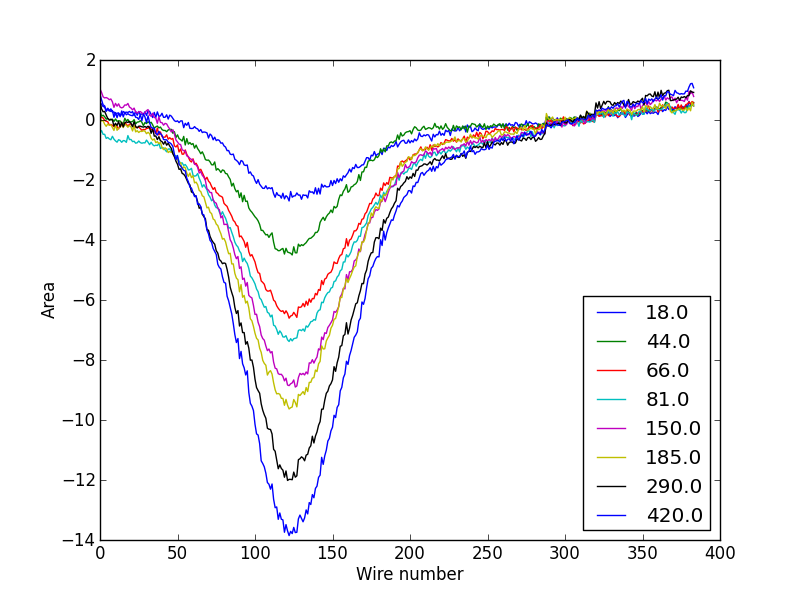
\includegraphics[width=0.55\textwidth]{./light_figures/PMT_xtalk_PE_plot.png}
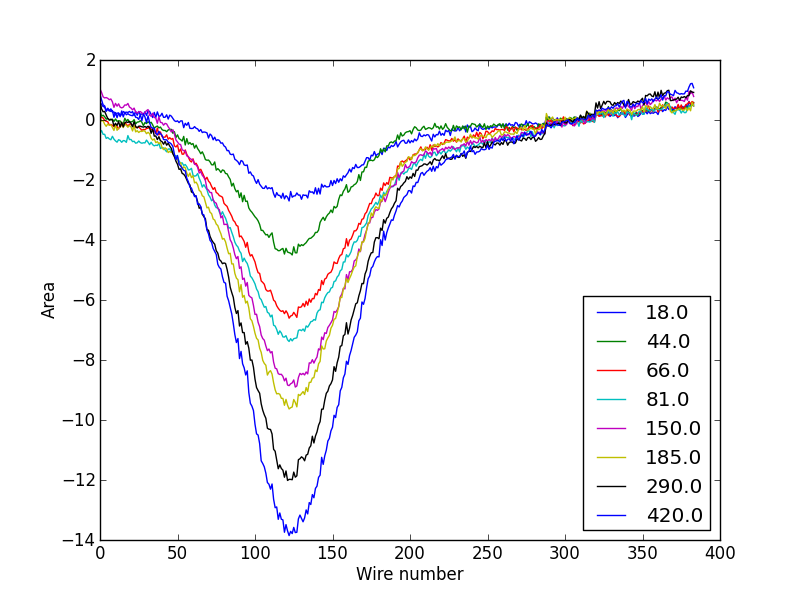
\includegraphics[width=0.55\textwidth]{./light_figures/PMT_xtalk_PE_plot.png}
\caption{Area of signal pulses recorded on collection plane (in arbitrary units) as a function of wire number (arb. offset). The legend indicates the calibrated photo-electron count. The signal pulses are averaged over 50,000 repetitions. The plots are pinned together at wire 300, as the distribution baseline fluctuated over the course of the experiment due to intermittent noise.
 \label{fig:PMTxtalk}  }
\end{figure}

The ICARUS detector has observed an unexpected cross-talk between their PMTs and collection wire plane \cite{Ankowski:2008aa}. The Argontube test stand at the University of Bern also observed this effect \cite{BernPrivate}.   Therefore, while the \lartpc was under final testing, before being rolled into the cryostat, an experiment was devised in order to determine the implication of this cross-talk for MicroBooNE.  One of the production $8''$ Hamamatsu R5912-02mod PMTs was placed $5''$ from the \lartpc collection wire plane. This PMT was encased in a dark box with an optical fiber delivering light from a LED flasher. The collection wire plane was read out using a DAQ test-stand that reflects the final DAQ design.

A clear signal was observed on the collection plane when the LED fired. The magnitude of the signal was characterized as a function of photo-electron count (figure~\ref{fig:PMTxtalk}) and separation between the PMT and wire-plane. The signal induced on the collection plane was estimated to be no more than $\sim10$ ADC counts for a cosmic ray under normal operating conditions. This was reduced to $\sim2$ ADC counts when the PMT was encased in the $\mu$-metal shields. This was deemed an acceptably small amount that further shielding was not required.

The effect appears to saturate with photo-electron count, and is reduced when shorting the resistors between the anode and last dynode. A later test with Argontube showed that the signal was drastically amplified when using capacitors not able to withstand cryogenic temperatures in the PMT base \cite{BernPrivate}. This suggests that the effect is electrostatic in nature, and probably due to capacitive coupling between the PMT and wire-plane.  This is also suggested by the similarity between the signals observed and those produced by anode-coupled readout of a light collection system \cite{Moss:2015hha}.

\subsection{Initial Performance of the MicroBooNE Light Collection System}

The system was first powered on after the cryostat had been filled with liquid argon.  All the PMTs in both the primary and secondary system were found to be operational.  Figure~\ref{fig:example_readout} shows the waveforms for all the PMT channels around the time that a large pulse, potentially from a cosmic ray muon, is observed.  After initial checks of the system's health, the single photoelectron response of each PMT was set such that a one photo-electron pulse has an amplitude of 20 ADC counts as seen by the PMT readout system.  The flasher LED system, described previously, is used to set this response. Figure~\ref{fig:example_spe_wfm} shows a candidate single photoelectron pulse following arrival of a TTL logic pulse driving the LED flasher system.  The LED light level is set so that the majority (about 80\%) of waveforms see no response in the region where pulses from the LED are expected to occur.  This ensures that for windows with pulses, the pulses are of single photoelectrons.  Figure~\ref{fig:example_spe_pulsedist} shows an example of the area vs. maximum amplitude of such pulses seen by a PMT during the flasher runs.

%\begin{figure}[t]
%\centering 
%\includegraphics[width=0.55\textwidth]{./light_figures/uboone_cosmic.jpg}
%\includegraphics[width=0.55\textwidth]{uboone_cosmic.jpg}
%\caption{First recorded waveforms from the MicroBooNE light collection system.  Image is of coincident pulses of light seen by two adjacent PMTs.  This signal is what one might expect for a cosmic ray muon crossing near the two PMTs.}
% \label{fig:example_uboonecosmic}
%\end{figure}

\begin{figure}[t]
\centering 
%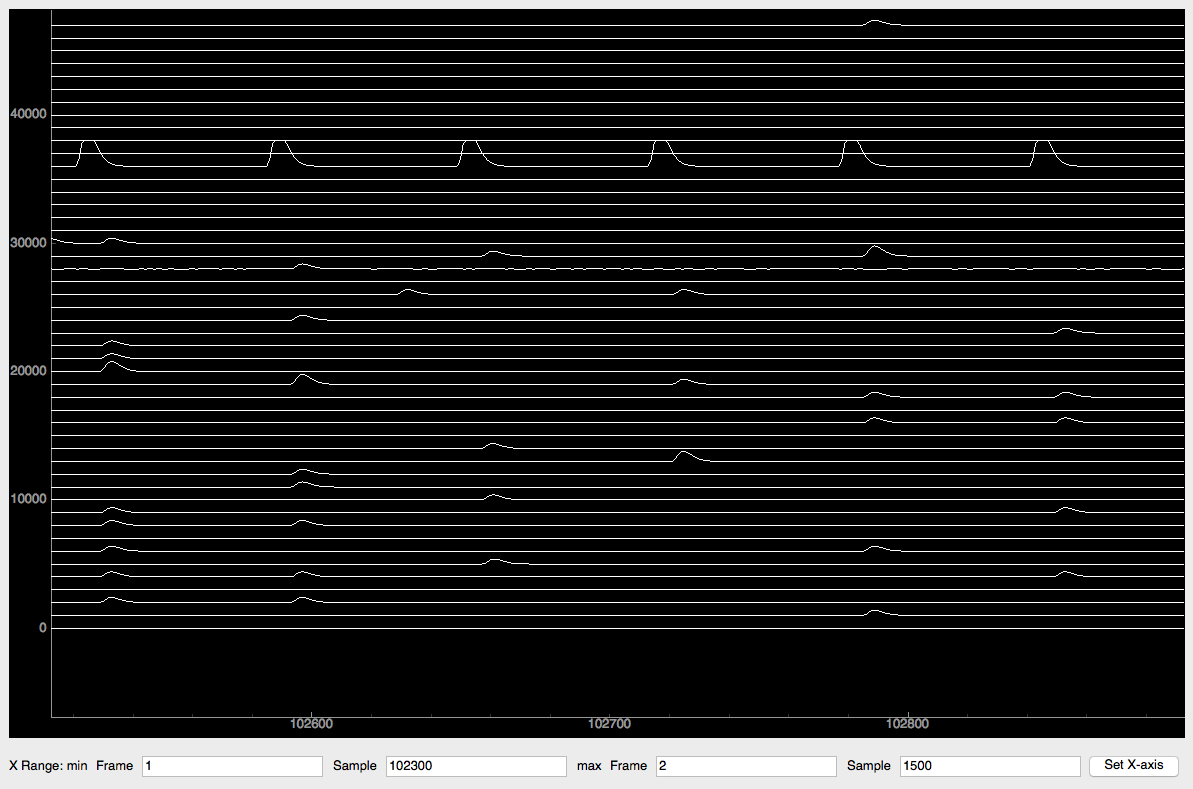
\includegraphics[width=0.95\textwidth]{./light_figures/flasher_mc_example_replaceme.png}
%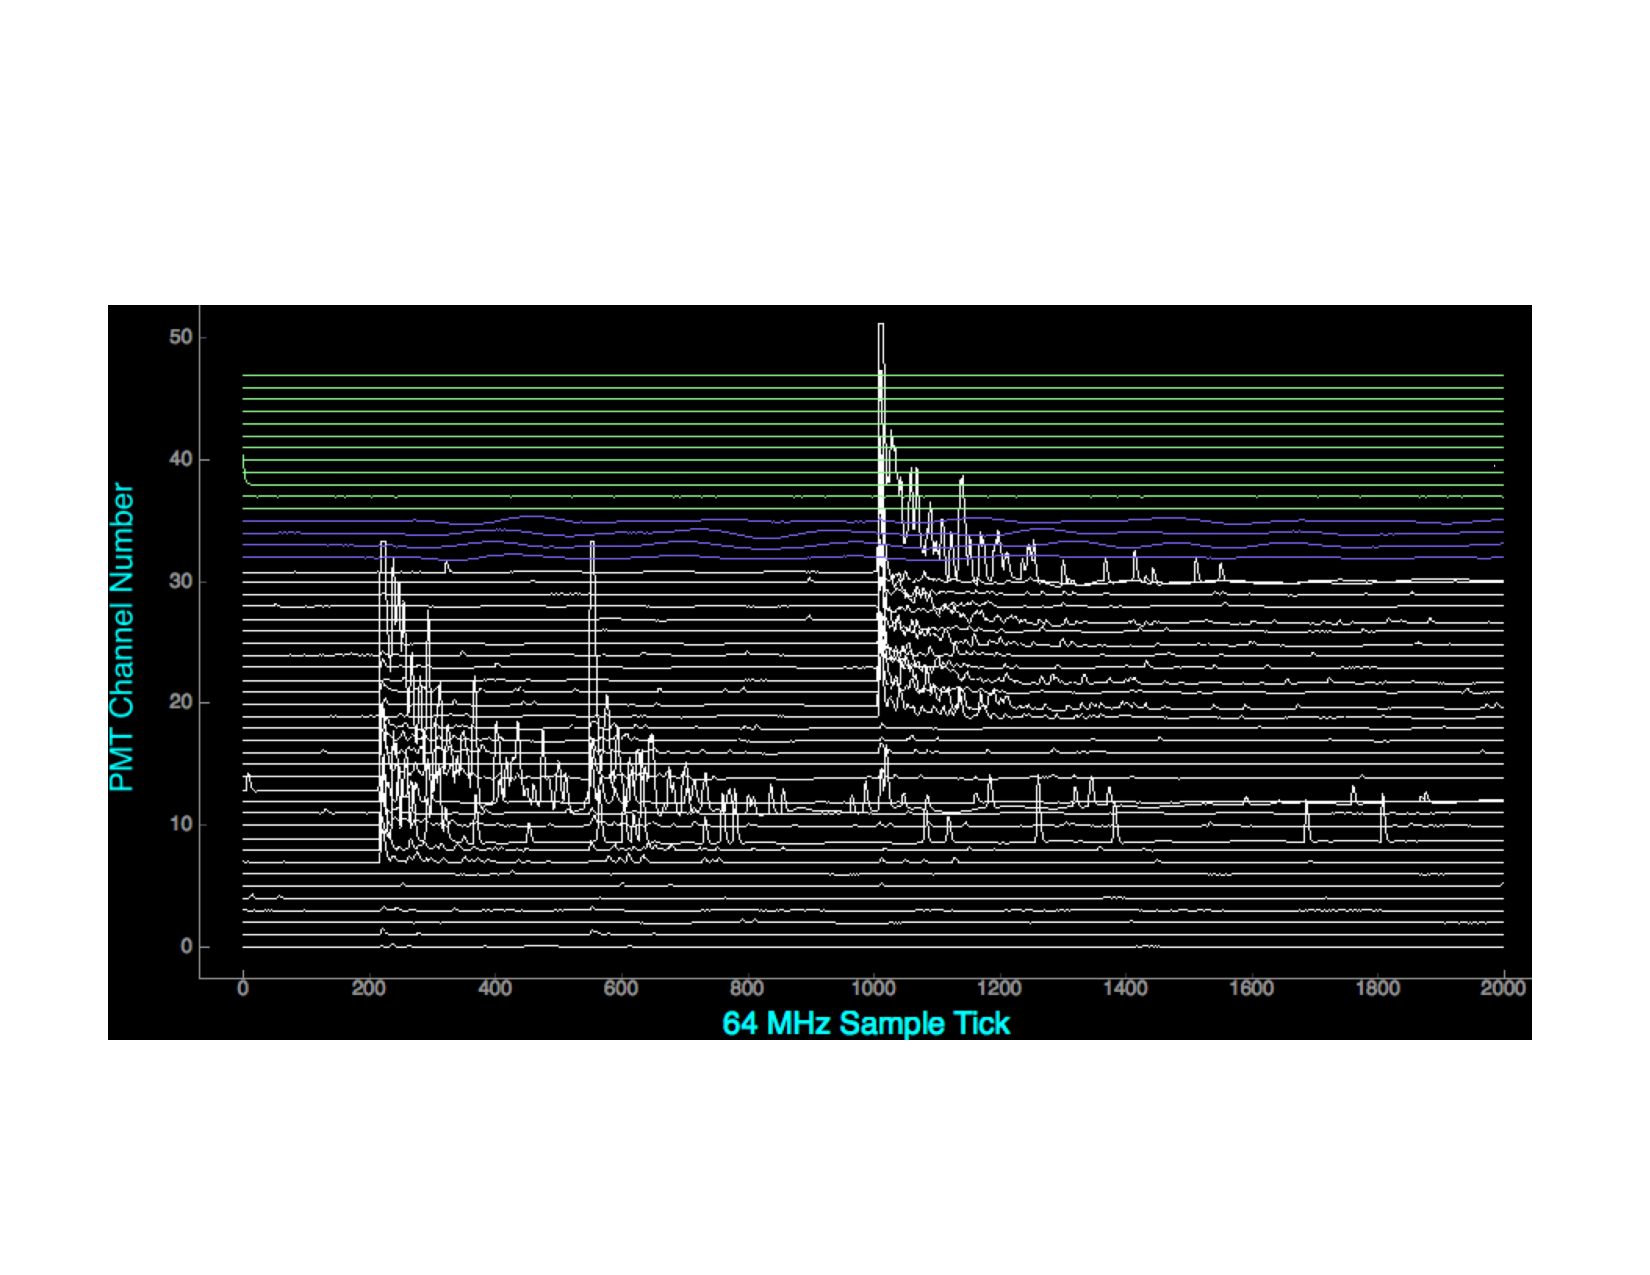
\includegraphics[width=0.95\textwidth]{pylard.pdf}
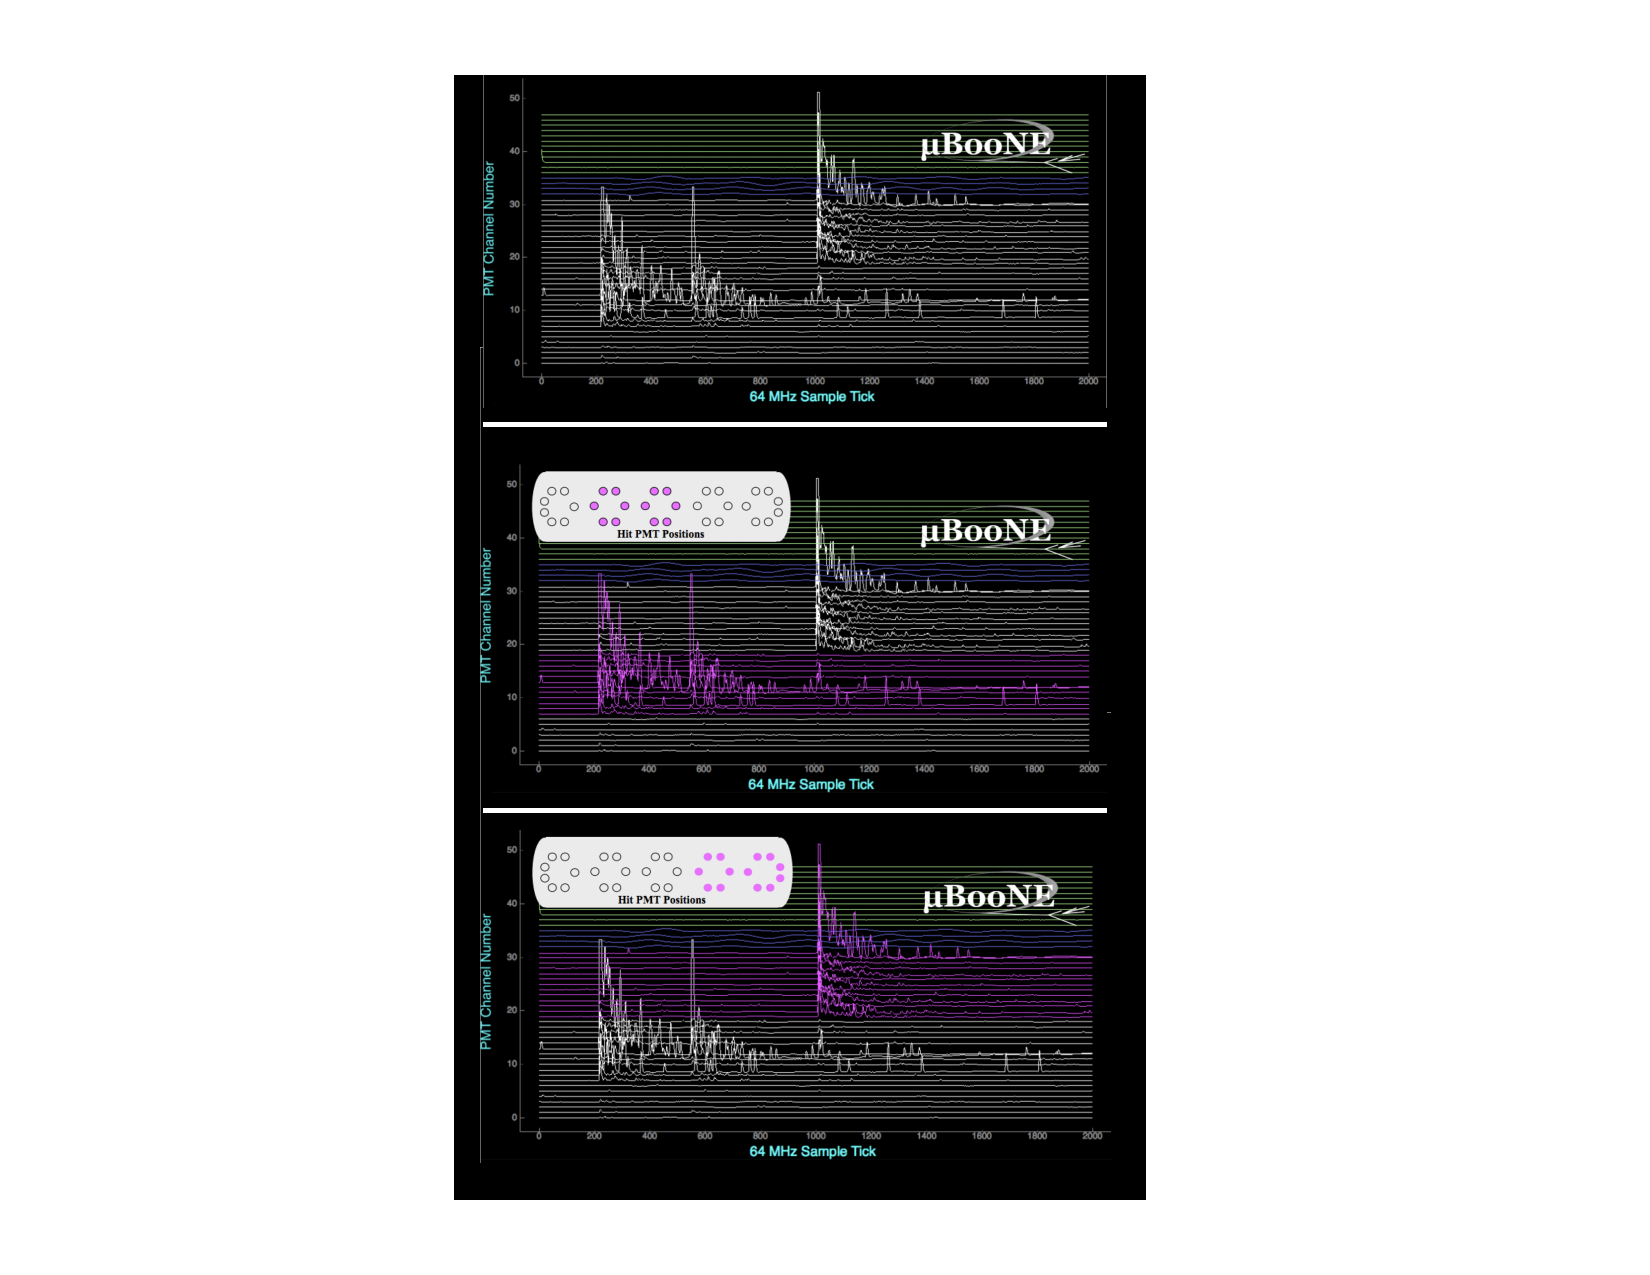
\includegraphics[height=0.7\textheight]{./light_figures/eventtriplet.pdf}
\caption{Top:  Example waveforms from all 32 PMTs of the primary light collection system over a 31.25 microsecond readout window.  The waveforms from the PMTs are in white.  The blue waveforms are from the secondary lightguide PMTs, which are off in this picture.  Waveforms from channels reserved for logic inputs are shown in green.  In this image, the PMTs see two successive flashes of light at different parts of the detector.  Middle and Bottom:   Magenta highlights the early and late pulse, with the insets showing the PMTs which fired.   Each pulse is likely from two cosmic ray muons traveling through the detector.}
 \label{fig:example_readout}
 \end{figure}

\begin{figure}[t]
\centering 
%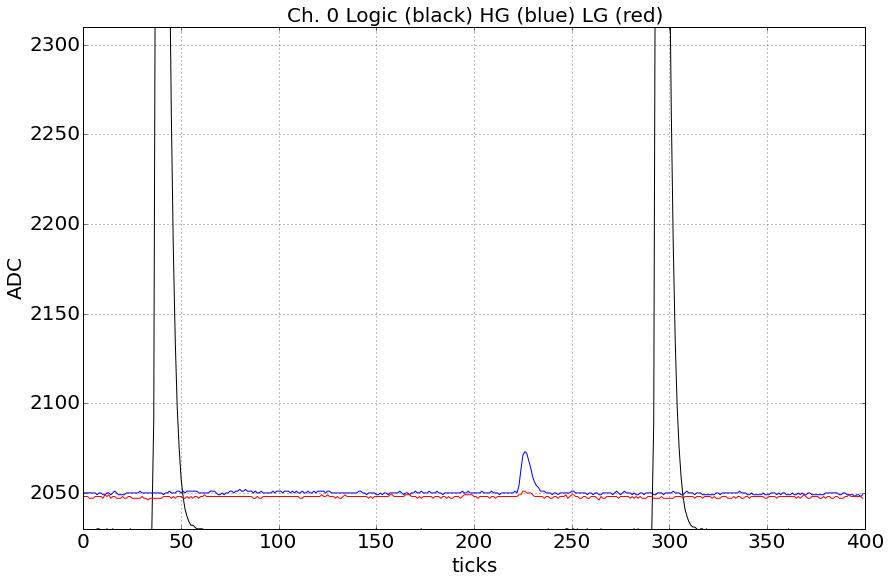
\includegraphics[width=0.55\textwidth]{./light_figures/sample_flasher_spe.png}
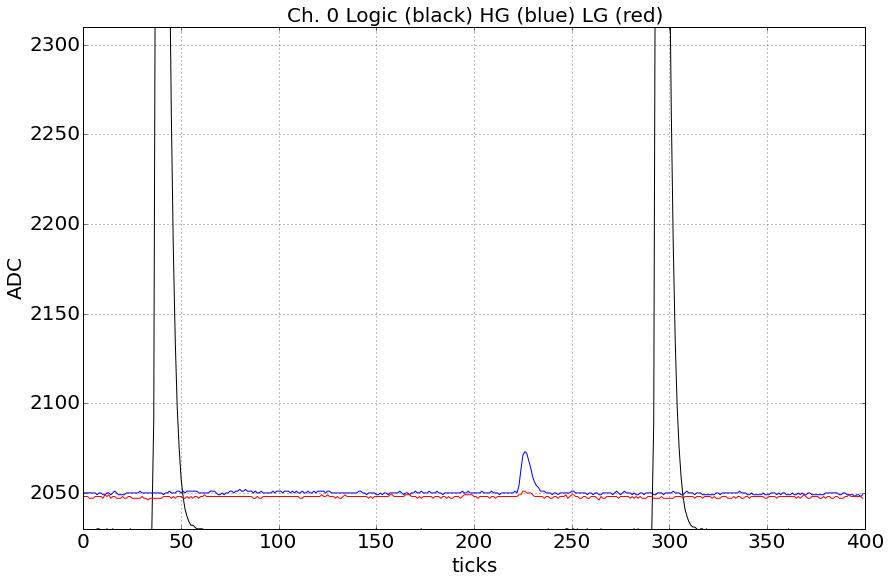
\includegraphics[width=0.55\textwidth]{./light_figures/sample_flasher_spe.png}
\caption{Example waveform captured by the PMT readout electronics during single photoelectron calibrations.  The black waveform is of logic pulses that mark time at which an LED in the flasher system is driven.  After some delay coming from PMT cable lengths and the flasher system, a candidate single photoelectron pulses is seen.}
 \label{fig:example_spe_wfm}
 \end{figure}


\begin{figure}[t]
\centering 
%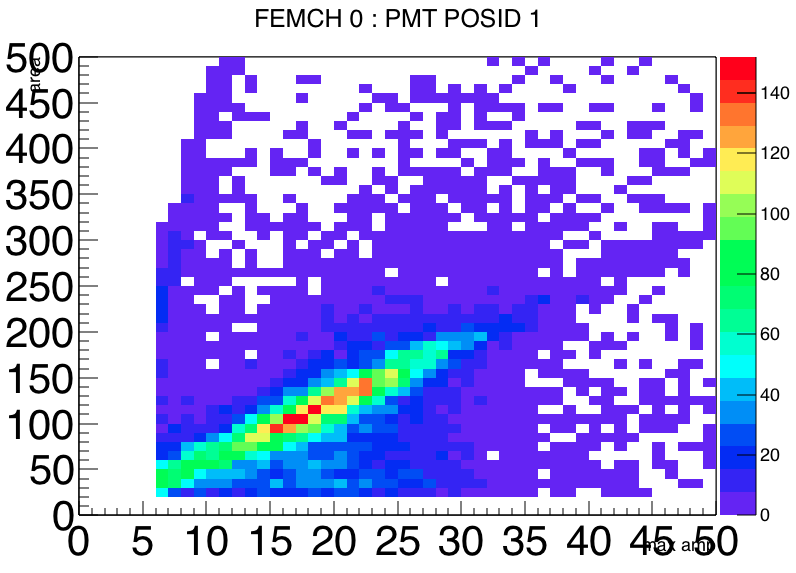
\includegraphics[width=0.55\textwidth]{./light_figures/h2_ch0_pmt1.png}
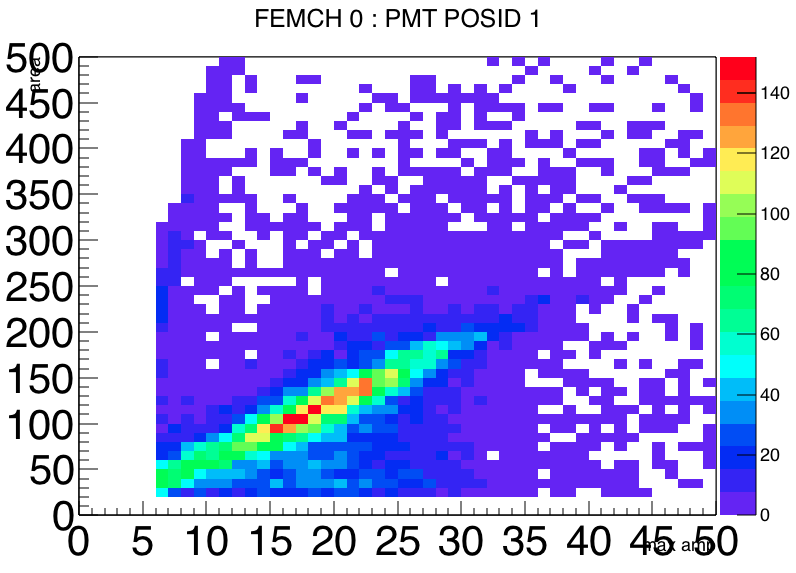
\includegraphics[width=0.55\textwidth]{./light_figures/h2_ch0_pmt1.png}
\caption{Distribution of the maximum amplitude and charge of pulses collected during an LED flasher calibration run. The central distribution of events is due to single photoelectron pulses.}
 \label{fig:example_spe_pulsedist} 
\end{figure}



%%%%%%%%%%%   bib entries  %%%%%%%%%%%%%%%%

%\bibitem{Amerio:2004ze} 
%  S.~Amerio {\it et al.} [ICARUS Collaboration],
%  ``Design, construction and tests of the ICARUS T600 detector,''
%  Nucl.\ Instrum.\ Meth.\ A {\bf 527}, 329 (2004).
%\bibitem{Bellamy:1994bv} 
%  E.~H.~Bellamy {\it et al.},
%  ``Absolute calibration and monitoring of a spectrometric channel using a photomultiplier,''
%  Nucl.\ Instrum.\ Meth.\ A {\bf 339}, 468 (1994).
%\bibitem{Meyer:2008qb} 
%  H.~O.~Meyer,
%  ``Dark Rate of a Photomultiplier at Cryogenic Temperatures,''
%  arXiv:0805.0771 [nucl-ex].
%
%\bibitem{Bugel:2011xg} 
%  L.~Bugel, J.~M.~Conrad, C.~Ignarra, B.~J.~P.~Jones, T.~Katori, T.~Smidt and H.-K.~Tanaka,
%  ``Demonstration of a Lightguide Detector for Liquid Argon TPCs,''
%  Nucl.\ Instrum.\ Meth.\ A {\bf 640}, 69 (2011)
%  [arXiv:1101.3013 [physics.ins-det]].
%\bibitem{Katori:2011uq} 
%  T.~Katori [MicroBooNE Collaboration],
%  ``MicroBooNE, A Liquid Argon Time Projection Chamber (LArTPC) Neutrino Experiment,''
%  AIP Conf.\ Proc.\  {\bf 1405}, 250 (2011)
%  [arXiv:1107.5112 [hep-ex]].
%\bibitem{Chiu:2012ju} 
%  C.~S.~Chiu, C.~Ignarra, L.~Bugel, H.~Chen, J.~M.~Conrad, B.~J.~P.~Jones, T.~Katori and I.~Moult,
%  ``Environmental Effects on TPB Wavelength-Shifting Coatings,''
%  JINST {\bf 7}, P07007 (2012)
%  [arXiv:1204.5762 [physics.ins-det]].
%\bibitem{Baptista:2012bf} 
%  B.~Baptista, L.~Bugel, C.~Chiu, J.~M.~Conrad, C.~M.~Ignarra, B.~J.~P.~Jones, T.~Katori and S.~Mufson,
%  ``Benchmarking TPB-coated Light Guides for Liquid Argon TPC Light Detection Systems,''
%  arXiv:1210.3793 [physics.ins-det].
%\bibitem{Briese:2013wua} 
%  T.~Briese, L.~Bugel, J.~M.~Conrad, M.~Fournier, C.~Ignarra, B.~J.~P.~Jones, T.~Katori and R.~Navarrete-Perez {\it et al.},
%``Testing of Cryogenic Photomultiplier Tubes for the MicroBooNE Experiment,''
%  JINST {\bf 8}, T07005 (2013)
%  [arXiv:1304.0821 [physics.ins-det]].
%\bibitem{Jones:2013bca} 
%  B.~J.~P.~Jones, C.~S.~Chiu, J.~M.~Conrad, C.~M.~Ignarra, T.~Katori and M.~Toups,
%  ``A Measurement of the Absorption of Liquid Argon Scintillation Light by Dissolved Nitrogen at the Part-Per-Million Level,''
%  JINST {\bf 8}, P07011 (2013)
%  [JINST {\bf 8}, E09001 (2013)]
%  [arXiv:1306.4605 [physics.ins-det]].
%\bibitem{Jones:2013mfa} 
%  B.~J.~P.~Jones {\it et al.},
%  ``The Effects of Dissolved Methane upon Liquid Argon Scintillation Light,''
%  JINST {\bf 8}, P12015 (2013)
%  [arXiv:1308.3658 [physics.ins-det]].  
%\bibitem{Katori:2013wqa} 
%  T.~Katori [MicroBooNE Collaboration],
%  ``The MicroBooNE light collection system,''
%  JINST {\bf 8}, C10011 (2013)
%  [arXiv:1307.5256 [physics.ins-det]].
%\bibitem{Bromberg:2013fla} 
%  B.~Baller {\it et al.},
%  ``Liquid Argon Time Projection Chamber Research and Development in the United States,''
%  JINST {\bf 9}, T05005 (2014)
%  [arXiv:1307.8166 [physics.ins-det]].
%\bibitem{Moss:2014ota} 
%  Z.~Moss, L.~Bugel, G.~Collin, J.~M.~Conrad, B.~J.~P.~Jones, J.~Moon, M.~Toups and T.~Wongjirad,
%  ``Improved TPB-coated Light Guides for Liquid Argon TPC Light Detection Systems,''
%  arXiv:1410.6256 [physics.ins-det].
%\bibitem{Conrad:2015xta} 
%  J.~Conrad {\it et al.} [MicroBooNE Collaboration],
%  ``The Photomultiplier Tube Calibration System of the MicroBooNE Experiment,''
%  JINST {\bf 10}, no. 06, T06001 (2015)
%  [arXiv:1502.04159 [physics.ins-det]].
%\bibitem{Acciarri:2015hha} 
%  R.~Acciarri {\it et al.},
%  ``Summary of the Second Workshop on Liquid Argon Time Projection Chamber Research and Development in the United States,''
%  arXiv:1504.05608 [physics.ins-det].
%\bibitem{Moss:2015hha} 
%  Z.~Moss, M.~Toups, L.~Bugel, G.~H.~Collin and J.~M.~Conrad,
%  ``Anode-Coupled Readout for Light Collection in Liquid Argon TPCs,''
%  arXiv:1507.01997 [physics.ins-det].
%  
%\bibitem{Icarus:0812}
%  A.~Ankowski {\it et al.},
%  ``Energy reconstruction of electromagnetic showers from $\pi^0$ decays with the ICARUS T600 Liquid Argon TPC,'' 
%  arXiv:0812.2373 [physics.ins-det].
%
%\end{thebibliography}

  

%@article{Amerio:2004ze,
%      author         = "Amerio, S. and others",
%      title          = "{Design, construction and tests of the ICARUS T600
%                        detector}",
%      collaboration  = "ICARUS",
%      journal        = "Nucl. Instrum. Meth.",
%      volume         = "A527",
%      year           = "2004",
%      pages          = "329-410",
%      doi            = "10.1016/j.nima.2004.02.044",
%      SLACcitation   = "%%CITATION = NUIMA,A527,329;%%"
%}
%@article{Bellamy:1994bv,
%      author         = "Bellamy, E. H. and Bellettini, G. and Gervelli, F. and
%                        Incagli, M. and Lucchesi, D. and Pagliarone, C. and Zetti,
%                        F. and Budagov, {\relax Yu}. and Chirikov-Zorin, I. and
%                        Tokar, S.",
%      title          = "{Absolute calibration and monitoring of a spectrometric
%                        channel using a photomultiplier}",
%      journal        = "Nucl. Instrum. Meth.",
%      volume         = "A339",
%      year           = "1994",
%      pages          = "468-476",
%      doi            = "10.1016/0168-9002(94)90183-X",
%      SLACcitation   = "%%CITATION = NUIMA,A339,468;%%"
%}
%@article{Meyer:2008qb,
%      author         = "Meyer, H. O.",
%      title          = "{Dark Rate of a Photomultiplier at Cryogenic
%                        Temperatures}",
%      year           = "2008",
%      eprint         = "0805.0771",
%      archivePrefix  = "arXiv",
%      primaryClass   = "nucl-ex",
%      SLACcitation   = "%%CITATION = ARXIV:0805.0771;%%"
%}
%
%
%
%
%
%  
%  
%
%
%  
%@article{Bugel:2011xg,
%      author         = "Bugel, L. and Conrad, J. M. and Ignarra, C. and Jones, B.
%                        J. P. and Katori, T. and Smidt, T. and Tanaka, H. -K.",
%      title          = "{Demonstration of a Lightguide Detector for Liquid Argon
%                        TPCs}",
%      journal        = "Nucl. Instrum. Meth.",
%      volume         = "A640",
%      year           = "2011",
%      pages          = "69-75",
%      doi            = "10.1016/j.nima.2011.03.003",
%      eprint         = "1101.3013",
%      archivePrefix  = "arXiv",
%      primaryClass   = "physics.ins-det",
%      SLACcitation   = "%%CITATION = ARXIV:1101.3013;%%"
%}
%@article{Katori:2011uq,
%      author         = "Katori, Teppei",
%      title          = "{MicroBooNE, A Liquid Argon Time Projection Chamber
%                        (LArTPC) Neutrino Experiment}",
%      booktitle      = "{Proceedings, 7th International Workshop on
%                        Neutrino-nucleus interactions in the few GeV region (NUINT
%                        11)}",
%      collaboration  = "MicroBooNE",
%      journal        = "AIP Conf. Proc.",
%      volume         = "1405",
%      year           = "2011",
%      pages          = "250-255",
%      doi            = "10.1063/1.3661595",
%      eprint         = "1107.5112",
%      archivePrefix  = "arXiv",
%      primaryClass   = "hep-ex",
%      reportNumber   = "FERMILAB-CONF-11-355-E-PPD",
%      SLACcitation   = "%%CITATION = ARXIV:1107.5112;%%"
%}
%@article{Chiu:2012ju,
%      author         = "Chiu, C. S. and Ignarra, C. and Bugel, L. and Chen, H.
%                        and Conrad, J. M. and Jones, B. J. P. and Katori, T. and
%                        Moult, I.",
%      title          = "{Environmental Effects on TPB Wavelength-Shifting
%                        Coatings}",
%      journal        = "JINST",
%      volume         = "7",
%      year           = "2012",
%      pages          = "P07007",
%      doi            = "10.1088/1748-0221/7/07/P07007",
%      eprint         = "1204.5762",
%      archivePrefix  = "arXiv",
%      primaryClass   = "physics.ins-det",
%      SLACcitation   = "%%CITATION = ARXIV:1204.5762;%%"
%}
%@article{Baptista:2012bf,
%      author         = "Baptista, B. and Bugel, L. and Chiu, C. and Conrad, J. M.
%                        and Ignarra, C. M. and Jones, B. J. P. and Katori, T. and
%                        Mufson, S.",
%      title          = "{Benchmarking TPB-coated Light Guides for Liquid Argon
%                        TPC Light Detection Systems}",
%      year           = "2012",
%      eprint         = "1210.3793",
%      archivePrefix  = "arXiv",
%      primaryClass   = "physics.ins-det",
%      SLACcitation   = "%%CITATION = ARXIV:1210.3793;%%"
%}
%@article{Briese:2013wua,
%      author         = "Briese, T. and Bugel, L. and Conrad, J.M. and Fournier,
%                        M. and Ignarra, C. and others",
%      title          = "{Testing of Cryogenic Photomultiplier Tubes for the
%                        MicroBooNE Experiment}",
%      journal        = "JINST",
%      volume         = "8",
%      pages          = "T07005",
%      doi            = "10.1088/1748-0221/8/07/T07005",
%      year           = "2013",
%      eprint         = "1304.0821",
%      archivePrefix  = "arXiv",
%      primaryClass   = "physics.ins-det",
%      SLACcitation   = "%%CITATION = ARXIV:1304.0821;%%",
%}
%@article{Jones:2013bca,
%      author         = "Jones, B.J.P. and Chiu, C.S. and Conrad, J.M. and
%                        Ignarra, C.M. and Katori, T. and others",
%      title          = "{A Measurement of the Absorption of Liquid Argon
%                        Scintillation Light by Dissolved Nitrogen at the
%                        Part-Per-Million Level}",
%      journal        = "JINST",
%      volume         = "8",
%      pages          = "P07011",
%      doi            = "10.1088/1748-0221/8/07/P07011,
%                        10.1088/1748-0221/8/09/E09001",
%      year           = "2013",
%      eprint         = "1306.4605",
%      archivePrefix  = "arXiv",
%      primaryClass   = "physics.ins-det",
%      reportNumber   = "FERMILAB-PUB-13-213-E",
%      SLACcitation   = "%%CITATION = ARXIV:1306.4605;%%",
%}
%@article{Jones:2013mfa,
%      author         = "Jones, B.J.P. and Alexander, T. and Back, H.O. and
%                        Collin, G. and Conrad, J.M. and others",
%      title          = "{The Effects of Dissolved Methane upon Liquid Argon
%                        Scintillation Light}",
%      journal        = "JINST",
%      volume         = "8",
%      pages          = "P12015",
%      doi            = "10.1088/1748-0221/8/12/P12015",
%      year           = "2013",
%      eprint         = "1308.3658",
%      archivePrefix  = "arXiv",
%      primaryClass   = "physics.ins-det",
%      reportNumber   = "FERMILAB-PUB-13-325-E-PPD",
%      SLACcitation   = "%%CITATION = ARXIV:1308.3658;%%",
%}
%@article{Katori:2013wqa,
%      author         = "Katori, Teppei",
%      title          = "{The MicroBooNE light collection system}",
%      collaboration  = "MicroBooNE",
%      journal        = "JINST",
%      volume         = "8",
%      pages          = "C10011",
%      doi            = "10.1088/1748-0221/8/10/C10011",
%      year           = "2013",
%      eprint         = "1307.5256",
%      archivePrefix  = "arXiv",
%      primaryClass   = "physics.ins-det",
%      SLACcitation   = "%%CITATION = ARXIV:1307.5256;%%",
%}
%@article{Bromberg:2013fla,
%      author         = "Baller, B. and Buchanan, N. and Cavanna, F. and Chen, H.
%                        and Church, E. and others",
%      title          = "{Liquid Argon Time Projection Chamber Research and
%                        Development in the United States}",
%      journal        = "JINST",
%      volume         = "9",
%      pages          = "T05005",
%      doi            = "10.1088/1748-0221/9/05/T05005",
%      year           = "2014",
%      eprint         = "1307.8166",
%      archivePrefix  = "arXiv",
%      primaryClass   = "physics.ins-det",
%      reportNumber   = "FERMILAB-CONF-13-257-E",
%      SLACcitation   = "%%CITATION = ARXIV:1307.8166;%%",
%}
%@article{Moss:2014ota,
%      author         = "Moss, Z. and Bugel, L. and Collin, G. and Conrad, J.M.
%                        and Jones, B.J.P. and others",
%      title          = "{Improved TPB-coated Light Guides for Liquid Argon TPC
%                        Light Detection Systems}",
%      year           = "2014",
%      eprint         = "1410.6256",
%      archivePrefix  = "arXiv",
%      primaryClass   = "physics.ins-det",
%      SLACcitation   = "%%CITATION = ARXIV:1410.6256;%%",
%}
%@article{Conrad:2015xta,
%      author         = "Conrad, J. and Jones, B.J.P. and Moss, Z. and Strauss, T.
%                        and Toups, M.",
%      title          = "{The Photomultiplier Tube Calibration System of the
%                        MicroBooNE Experiment}",
%      collaboration  = "MicroBooNE",
%      journal        = "JINST",
%      number         = "06",
%      volume         = "10",
%      pages          = "T06001",
%      doi            = "10.1088/1748-0221/10/06/T06001",
%      year           = "2015",
%      eprint         = "1502.04159",
%      archivePrefix  = "arXiv",
%      primaryClass   = "physics.ins-det",
%      reportNumber   = "FERMILAB-PUB-15-036-ND",
%      SLACcitation   = "%%CITATION = ARXIV:1502.04159;%%",
%} 
%  @article{Acciarri:2015hha,
%      author         = "Acciarri, R. and Adamowski, M. and Artrip, D. and Baller,
%                        B. and Bromberg, C. and others",
%      title          = "{Summary of the Second Workshop on Liquid Argon Time
%                        Projection Chamber Research and Development in the United
%                        States}",
%      year           = "2015",
%      eprint         = "1504.05608",
%      archivePrefix  = "arXiv",
%      primaryClass   = "physics.ins-det",
%      reportNumber   = "FERMILAB-CONF-15-149-ND",
%      SLACcitation   = "%%CITATION = ARXIV:1504.05608;%%",
%}
%  @article{Moss:2015hha,
%      author         = "Moss, Z. and Toups, M. and Bugel, L. and Collin, G.H. and
%                        Conrad, J.M.",
%      title          = "{Anode-Coupled Readout for Light Collection in Liquid
%                        Argon TPCs}",
%      year           = "2015",
%      eprint         = "1507.01997",
%      archivePrefix  = "arXiv",
%      primaryClass   = "physics.ins-det",
%      SLACcitation   = "%%CITATION = ARXIV:1507.01997;%%",
%}
%  @article{MeyerDark,
%      author         = "Meyer, H.O.",
%      title          = "{Spontaneous electron emission from a cold surface}",
%      journal        = "EPL",
%      number         = "89",
%      pages          = "58001",
%      doi            = "10.1209/0295-5075/89/58001",
%      year           = "2010",
%}
%
%
%
%
%@article{Moss:2015hha,
%      author         = "Moss, Z. and Toups, M. and Bugel, L. and Collin, G. H.
%                        and Conrad, J. M.",
%      title          = "{Anode-Coupled Readout for Light Collection in Liquid
%                        Argon TPCs}",
%      year           = "2015",
%      eprint         = "1507.01997",
%      archivePrefix  = "arXiv",
%      primaryClass   = "physics.ins-det",
%      SLACcitation   = "%%CITATION = ARXIV:1507.01997;%%"
%}
%
%
%
%@article{HamamatsuBook,
%      author         = "{Hamamatsu Photonics}",
%      title          = "{Photomultiplier Tubes, Basics and Applications, Third Edition, Chapter 13.9}",
%      year           = "2007",
%      note           = "{https://www.hamamatsu.com/resources/pdf/etd/PMT_handbook_v3aE.pdf}",
%}
